\documentclass{NauThesis}

\usepackage{algorithmic}
\usepackage{algorithm}
\usepackage{amsmath}
\usepackage{natbib}
% \usepackage{tabularx} 
\DeclareMathOperator*{\argmin}{arg\,min}
\setcitestyle{numbers,square}

\begin{document}
\ZhCover{MG2108129}{一种鲁棒的基于特征子空间插值\\的数据合成方法}{统计与数据科学学院}{统计学}{机器学习、数据挖掘}{学术硕士}{杜玉坤}{苍玉权、陆敏教授}{2023.05.17}
\EnCover{A Robust Data Synthesis Method based on Feature Subspace Interpolation}{Academic}{Mathematical Statistics}{DU Yukun}{Professor Cang Yuquan; Lu min}{Statistics and Data Science}{February 2024}
\Statement

\begin{ZhAbstract}
    数据噪音是指在数据收集、处理或传输过程中引入的任何错误或无关信息,会显著影响数据分析的结果以及模型的泛化能力。特别是在高维数据和稀疏样本中,数据噪音会加剧过拟合的风险从而降低预测性能。因此,解决数据噪音问题不仅有助于提高模型的预测性能,还可以增强模型的鲁棒性,使其更能适应实际应用场景的需求。然而,目前的数据噪音处理方法,如数据清洗、数据平滑、噪音识别技术等,虽然可以减少数据中的随机波动,但也可能导致数据过度泛化。这种过度泛化可能会模糊数据中的重要特征和细节,从而影响数据分析与预测的准确性。
\\\hspace*{2em}在这种背景下,本文提出了一种创新的对于含噪数据集处理的数据合成方法,基于特征子空间插值的思想,命名为RSIS(Robust Subspace Interpolation Synthesis)。这种方法可以从两方面对样本进行优化:首先,RSIS方法可以合成误差较小的样本以降低原始数据集平均误差,并且减小了大误差样本的占比;其次,由于RSIS方法是在特征子空间之间进行多次等距且线性插值的,该方法可以提升原始数据的多样性以及代表性,从而增强了变量之间的函数映射关系。即使数据集中含有不同分布的噪音,RSIS依旧可以达到很好的优化效果。与传统的噪声处理方法相比,RSIS更适用于机器学习领域的样本噪音处理,即使是在处理含有未知复杂噪音的高维数据时,也可以有效提升机器学习模型的泛化能力。
\\\hspace*{2em}本文在理论上证明了噪音不同分布下RSIS方法的有效性,并且在模拟实验中通过威尔科克森符号秩检验得到了进一步验证。RSIS方法在实例数据上的实验结果表明,该方法可以适用于多种模型,显著优化模型的预测能力。并且即使面对大方差噪音以及违背RSIS方法假设情况下,RSIS依旧表现出良好的鲁棒性。此外,本文将RSIS方法引入到卷积神经网络框架中,同样可以有效提升图像分类模型的预测效果。
    \ZhKeywords 特征子空间;鲁棒性;数据合成;线性等距插值;优化样本
\end{ZhAbstract}

\begin{EnAbstract}
    Data noise, referring to any errors or irrelevant information introduced during data collection, processing, or transmission, poses a significant challenge to the accuracy of prediction models and data analysis. Noise can substantially distort the outcomes of data analysis, leading to biases in model training and affecting the models' generalization capabilities for unseen data. Hence, addressing data noise not only aids in enhancing the accuracy of model predictions but also strengthens model robustness, making it more adaptable to real-world application requirements. However, current methods for handling data noise, such as data cleaning, smoothing, and noise detection techniques, while reducing random fluctuations in data, may also lead to overgeneralization. This overgeneralization could obscure important features and details in the data, thus affecting the accuracy of data analysis and prediction.
    \\\hspace*{2em}Against this backdrop, this paper introduces an innovative data synthesis method for processing noisy datasets, termed RSIS (Robust Subspace Interpolation Synthesis), grounded on the concept of feature subspace interpolation. This method optimizes samples in two ways: firstly, the RSIS approach synthesizes samples with smaller errors to reduce the average error of the original dataset and decrease the proportion of large-error samples; secondly, as the RSIS method performs multiple equidistant and linear interpolations between feature subspaces, it enhances the diversity and representativeness of the original data, thereby strengthening the functional mapping relationships between variables. Even with noise of varying distributions within the dataset, RSIS still achieves excellent optimization results. Compared to traditional noise handling methods, RSIS is more suited for sample noise processing in the machine learning domain, effectively enhancing the generalization capabilities of machine learning models, even when dealing with high-dimensional data containing unknown complex noise.
    \\\hspace*{2em}This paper theoretically demonstrates the effectiveness of the RSIS method under different noise distributions and further validates it through simulation experiments using the Wilcoxon signed-rank test. Experimental results on example data reveal that the method is applicable to various models, significantly optimizing their predictive capabilities. Moreover, RSIS exhibits commendable robustness even in the face of large-variance noise and under conditions that deviate from the RSIS assumptions. Additionally, incorporating the RSIS approach into the convolutional neural network framework effectively enhances the predictive performance of image classification models.
    \EnKeywords Subspace, Robust, Data Synthesis, Linear and Equidistant Interpolation, Sample Optimization
\end{EnAbstract}


\TableOfContents

\mainpagestyle
\setcounter{page}{1}

\chapter{绪言}

\section{研究背景及意义}
数据噪声指的是数据中的任何不准确、不相关或误导性信息,可能源于多种原因,如仪器误差、数据录入错误、传输问题,甚至是数据采集过程中的系统性偏差\cite{ref1,ref2}。在大多数实际问题中,噪声的分布都是复杂且未知的,这些噪声可能导致数据分析和机器学习模型的性能大打折扣,尤其是在需要高度精准预测和分析的应用场景中,如医疗影像分析、金融市场预测、环境监测等\cite{ref4,ref5,ref6}。在这些领域,即使是微小的数据误差也可能导致严重的后果。因此,有效地识别和处理数据中的噪声,已成为提高预测模型准确性和可靠性的关键步骤。
\\\hspace*{2em}为了解决数据噪音的问题,研究者们开发了多种方法,包括数据清洗\cite{ref7,ref8}、数据平滑\cite{ref9,ref10,ref11}和异常值检测\cite{ref12,ref13}等。这些方法主要集中于减轻或移除数据中的噪声,但它们通常不会从根本上提升数据质量。例如,数据清洗过程可能难以判断数据噪声与真实的异常值。异常值在某些情况下可能是数据分析中的重要信息源,但数据清洗可能错误地将其视为噪声并将其移除,从而可能导致关键信息的损失\cite{ref14}。同样的,数据平滑技术,如移动平均或高斯平滑,虽然可以减少数据中的随机波动,但也可能导致数据过度泛化。这种过度泛化可能会模糊数据中的重要特征和细节,从而影响数据分析的准确性\cite{ref15}。此外,当处理复杂以及高维度的噪音数据集时,传统的噪声处理方法具有局限性。在高维数据中,噪声和有用信息之间的界限可能更加模糊,有效地识别和处理噪声变得更加困难,这就会导致在降噪过程中可能误删掉有价值的数据,或者保留过多的噪声。
\\\hspace*{2em}在这种背景下,本文提出了一种创新的可对含噪数据集优化的数据合成方法,基于特征子空间插值的思想,命名为RSIS(Robust Subspace Interpolation Synthesis)。这种方法可以从两方面对原始样本进行优化:首先在不损失样本原始信息的前提下,通过合成误差较小的样本,降低数据集整体的噪音水平,并减少高噪音样本的比例;其次,RSIS通过特征子空间等距且线性的插值,合成了更多具有代表性、多样性的样本,强化了数据集变量之间真实的函数映射关系。与传统的含噪数据集噪声处理方法相比,RSIS更适用于机器学习领域的样本噪音处理,即使是在处理含有未知复杂噪音的高纬数据时,该方法也可以有效提升机器学习模型的泛化能力。
\\\hspace*{2em}RSIS方法包含几个关键步骤。首先,对原始数据集进行迭代层次聚类,该方法可以将原始数据集划分为多个样本量相近的子集,这一步骤会将原始特征空间划分为多个具有相近样本量的子空间;其次,根据聚类结果,RSIS方法引入了旅行商问题的思想对特征子空间进行排序;随后,本文结合了软参数多任务学习的机制,根据排序结果对相邻子空间之间进行考虑了全局信息的线性拟合;最后,本文提出了一种创新的多阶段最小权匹配启发式方法,通过该方法可以得到一种较优的插值匹配策略,通过该策略对样本进行线性插值可以生成具有较小误差的样本。
\\\hspace*{2em}目前许多研究都假设样本的噪音是同分布的,但是这种情况对于实际应用中是较为少见的,本文从理论上证明了RSIS方法即使面对不同分布的噪音样本依旧可以表现出很好的优化效果。基于噪音不同分布的场景,本文还模拟了样本中含有未知且不同分布的复杂噪音的情况,RSIS方法在实际模拟实验中依旧可以具有良好的鲁棒性,并且对样本进行显著的优化。此外,本文还将RSIS方法结合卷机神经网络应用到计算机视觉领域,通过实验结果可知,RSIS方法同样可以有效提升图像分类模型的泛化能力。

\section{研究现状}
当前的数据合成技术致力于通过创造既非真实又在统计层面具备充分代表性的数据,来执行数据的增强、样本的扩充以及真实情景的模拟。这类方法在多个领域得到广泛应用,特别是在面临数据匮乏、需要严格隐私保护或进行复杂模型训练时显得尤为重要。以医疗行业为例,由于该领域对数据隐私的高度敏感性,合成数据技术便成为研究人员的有力工具。通过这种技术,他们能够在不泄露任何个人敏感信息的情况下,利用模型训练显著提升对疾病的诊断精度和效率\cite{ref16,ref17}。这不仅保证了研究活动的合法性和多样性的充分体现,而且促进了医学科研的进步和技术创新,为未来的医疗健康发展开辟新径。通过这种方式,合成数据技术在支持科学研究的同时,也为保护个人隐私提供了坚实的保障,展现了其在现代科技领域内不可或缺的价值。
\subsection{基于规则的方法}
基于规则的数据合成方法,通过严格遵循既定的算法或规则框架,能够在不损害数据质量的前提下,有效地生成新的数据实例或对现有数据进行适当的修改和补充。这类方法的应用广泛,如线性插值和多项式插值,利用已知数据点来估计未知点\cite{ref18,ref19};再比如复杂的图像数据增强技术,在处理图像数据时,数据增强技术通过应用一系列图像变换操作,如旋转、缩放、翻转等,有效地增加了训练集的多样性,这对于防止模型过拟合,提高模型对新未见数据的识别能力至关重要。此外,MixUp和CutMix等创新技术通过混合不同图像样本,生成新颖的、具有挑战性的数据样本,进一步推动模型泛化能力的提升\cite{ref20,ref21}。在更为复杂的系统分析和数据模拟领域,蒙特卡洛模拟和代理模型等方法通过简化的数学表达或随机抽样技术,能够精确地捕捉和模拟现实世界数据的分布特征,这对于理解复杂系统的动态行为、预测系统未来可能的状态变化,乃至于优化系统设计,都提供了强有力的支持\cite{ref22,ref23,ref24}。在当今数据驱动的科学研究和工程实践中,这些基于规则的数据合成方法已成为不可或缺的工具,它们不仅加速了数据分析的进程,也大幅度提升了研究和设计的效率与准确性。
\subsection{基于统计的方法}
在现代数据科学领域,基于统计的方法可以细分为参数方法和非参数方法,它们通过应用统计模型对数据分布进行估计,以此作为生成新数据的基础。参数方法主要依靠对数据分布的先验假设,通过设定特定的分布形式(如高斯混合模型、贝叶斯网络等)来生成新的数据\cite{ref25,ref26}。这类方法认为数据遵循特定的概率分布(例如正态分布、泊松分布等),并据此生成新的数据点,这种方式在保持数据内部相关性的同时,尝试复现原始数据集的统计特性。然而,参数方法的效果很大程度上受到模型假设准确性的影响,因此,对数据的分布特征有一定的了解和判断变得尤为关键\cite{ref27,ref28,ref29}。
\\\hspace*{2em}相较于严格定义数据分布的参数方法,非参数方法以其灵活性和适应性也得到了广泛的应用。这类方法并不假定数据遵循任何特定的数学分布,而是依据数据本身的特性来推断其分布形态。例如,直方图方法依赖于数据本身的频率分布来估计整体分布,而核密度估计(KDE)则通过平滑处理来估计概率密度函数,这两种方法均能有效捕捉和模拟数据的分布特性,即使在数据复杂多变的情况下也不例外\cite{ref30,ref31}。该领域中,较为著名的还有SMOTE(Synthetic Minority Over-sampling Technique)及其变体如SVMSMOTE和SMOTE-ENC,通过在少数类样本之间插值生成新样本,旨在解决数据不平衡问题。这种基于数据实例的合成方法不仅提高了模型对少数类的识别能力,也增强了模型对不同数据分布的适应性和泛化能力\cite{ref32,ref33}。特别是在面对不均衡数据集时,非参数方法能够通过合成少数类数据来平衡类别分布,进而提高分类模型的准确性和鲁棒性。在实际应用中,非参数方法的灵活性使其能够适应各种复杂且多变的数据环境。无论是自然界中的生物多样性数据,还是社会科学领域的人口统计数据,或是医学研究中的患者健康记录,非参数方法都能够根据数据本身的分布特征进行有效的数据合成和分析。此外,这类方法对于处理大规模数据集尤为有效,它能够从庞大的数据量中自动提取和学习数据的内在结构,为数据分析和模型训练提供了强大的支持\cite{ref34}。
\subsection{基于机器学习的方法}
近年来,基于机器学习的数据合成方法取得了飞速的发展,尤其是随着生成对抗网络(GANs)、变分自编码器(VAEs)和条件生成对抗网络(cGANs)等技术的出现。生成对抗网络通过引入一种创新性的训练框架,即生成器和判别器之间的对抗过程,极大地推动了数据合成技术的进步。生成器试图生成尽可能真实的数据以欺骗判别器,而判别器则尝试区分真实数据与生成数据,这种动态对抗过程促使生成器不断优化,从而生成高质量的合成数据。这一方法已被广泛应用于图像合成、文本生成和语音合成等领域,展现了其在多模态数据合成中的强大潜力\cite{ref35,ref36,ref37}。变分自编码器作为一种深度学习模型,通过引入潜在变量来学习数据的高维分布,使得VAEs能够在生成过程中考虑到数据内在的复杂结构。这不仅使得VAEs在图像去噪、风格转换和特征学习等任务中表现出色,也使其成为理解和分析复杂数据分布的有力工具\cite{ref38,ref39}。\\\hspace*{2em}条件生成对抗网络进一步扩展了GANs的应用范围,通过条件变量引导数据生成过程,使得模型能够根据指定的条件生成相应的数据。这种方法在个性化推荐、目标驱动的图像合成和语音到语音转换等领域展现了巨大的应用潜力,为数据合成提供了更高的灵活性和定制化能力\cite{ref40,ref41}。\\\hspace*{2em}此外,像PixelRNN和PixelCNN这样的自回归模型,通过学习数据的序列依赖性,逐步生成数据,从而在确保生成内容的连贯性和逻辑性方面发挥了关键作用。这类模型尤其适用于需要维持序列结构的数据生成任务,如文本生成、语音合成和图像填充等,为顺序数据的合成提供了一种有效的解决方案\cite{ref42,ref43,ref44}。\\\hspace*{2em}总体而言,这些基于机器学习的数据合成方法不仅推动了数据合成技术的发展,也为数据增强、模型训练和科学研究等领域提供了新的视角和工具,展现了深度学习在数据科学领域内日益增长的影响力和应用范围。
\subsection{基于混合的方法}
混合数据合成方法是在现代数据科学中应用广泛的一类技术,它们通过融合多种数据合成技术来提升合成数据的质量、多样性和实用性。这类方法特别适用于处理大规模、高维度和复杂结构的数据集,能够在保护数据隐私的同时,为数据分析和机器学习模型训练提供丰富的资源。\\\hspace*{2em}贝叶斯高斯混合模型(Bayesian GMM)采用贝叶斯推断方法来估计高斯混合模型的参数,与传统的最大似然估计方法相比,贝叶斯方法提供了一种更加灵活和全面的参数估计框架。通过引入先验知识和计算参数的后验分布,贝叶斯GMM能够更准确地表达参数的不确定性,从而在模拟复杂数据分布时表现出更高的灵活性和鲁棒性\cite{ref45,ref46}。这种方法尤其适用于那些参数分布未知或具有复杂结构的数据集,能够有效地捕捉数据内在的多模态特性。\\\hspace*{2em}狄利克雷过程混合模型(DPMM)是一种基于非参数贝叶斯方法的数据合成技术,它通过引入狄利克雷过程作为混合组分的先验分布,允许模型自动调整混合组件的数量。DPMM不仅能够根据数据自适应地确定潜在类别的数量,而且能够更准确地模拟数据的真实分布,生成与原始数据具有相似复杂结构的合成数据\cite{ref47,ref48}。这种灵活性使得DPMM在处理具有未知或无限潜在子群体的数据集时具有显著优势,如社会科学、生物信息学和市场研究等领域。\\\hspace*{2em}层次混合模型(HMM)通过引入层次结构来进一步增强数据合成的能力,它允许模型在不同的层次上捕捉数据的可变性和复杂性。通过模拟数据内在的层次关系,HMM能够生成更加贴近真实世界数据的合成样本\cite{ref49,ref50}。这种方法尤其适合于那些具有明显层次或组织结构的数据,比如医疗健康记录、社会网络数据以及自然语言文本。HMM不仅提高了合成数据的真实性和可信度,还为复杂数据分析提供了更深入的见解。\\\hspace*{2em}综上所述,混合数据合成方法通过整合贝叶斯高斯混合模型、狄利克雷过程混合模型和层次混合模型等先进技术,不仅提升了合成数据的质量和多样性,而且拓宽了数据合成在众多领域的应用。这些方法的发展为数据隐私保护、机器学习模型的鲁棒性训练以及复杂系统分析提供了新的可能性,标志着数据合成技术向更高级别的精确度和实用性迈进。
\section{主要研究内容}
本文提出了一种创新的对于含噪数据集优化的数据合成方法,基于特征子空间插值的思想,命名为RSIS方法。该方法融合了运筹优化、数据挖掘、机器学习多个学科技术,可以在保证不损害样本原始信息的前提下,合成大量具有较小误差的样本,从而提升机器学习模型的泛化能力。本文对RSIS方法进行了全面的模拟研究,通过生成含有复杂且未知噪音的数据集,本文探究了RSIS方法对于含噪数据集的优化效果以及RSIS方法中超参数的分析。在实例数据中,将经过RSIS优化后的样本用于机器学习实际的预测场景中,实验结果表明该方法可以显著提升模型的泛化能力。并且本文还将RSIS方法应用到计算机视觉领域进行拓展研究,创新地RSIS方法与卷积神经网络相结合,实验结果表明RSIS方法同样可以显著提升模型在图像分类任务的预测效果。本文剩余的章节安排如下:
\\\hspace*{2em}第二章节,由于RSIS方法融合了运筹优化、机器学习等多个领域的技术,本章节主要阐述了后续研究涉及到的相关概念,包括对于旅行商问题的阐述,卷积神经网络的详细介绍等。
\\\hspace*{2em}第三章节,将RSIS方法分为四个部分进行介绍。第一部分,主要介绍了一种无监督聚类算法,该算法可以通过较少的运算达到特征空间分割的目的,得到多个具有样本量相近的特征子空间。第二部分,主要解决了针对多个特征子空间的插值排序问题,将原始问题转化为旅行商问题进行求解。第三部分,融合了软参数共享机制,提出了针对两个相邻的子空间之间样本的线性拟合方法。第四部分,提出了一种创新的多阶段最小权样本匹配算法,基于加权二分图的最小权匹配问题的思想,针对两个相邻子空间之间的样本进行线性插值,通过匈牙利算法求解得到较优的样本插值匹配方案。在本章节的最后总结了RSIS方法的假设以及整体操作流程。
\\\hspace*{2em}第四章节,对RSIS方法进行模拟实验,本文通过生成含有复杂且未知噪音的数据集,探究了RSIS方法对于含噪数据集的优化效果。随后,选取了多个实例数据集,将RSIS方法结合机器学习模型对模型的泛化能力的提升进行详细探究,涉及到的模型有:多层感知机、梯度提升树、K近邻回归等。
\\\hspace*{2em}第五章节,将RSIS方法结合了CNN模型框架,探究RSIS方法对于特征提取后的张量数据的优化效果,并且考虑到了轻量型和非轻量网络,选择了ResNet、SqueezeNet、VGG等多个框架进行对比研究。
\\\hspace*{2em}第六章节,对本文进行了总结,论述了目前RSIS方法的不足,并且展望了对于RSIS方法未来的研究方向。
\section{本文创新}
目前已有的数据合成方法对于噪音数据集并不具有良好的鲁棒性,因为大部分数据合成方法的设计初衷并不是用于处理样本噪音的问题,如SMOTE算法,其目的是为了针对分类任务用于平衡样本数据;以及差分隐私算法是一种旨在提供强大隐私保护的技术,同时允许对数据集进行有用的统计分析\cite{ref32,ref51}。RSIS作为一种创新的基于混合方法的数据合成方法,不仅解决了含噪数据集的特定问题,也通过创新的合成技术来优化数据质量,进而提升机器学习模型在处理复杂数据时的性能和泛化能力。
\\\hspace*{2em}RSIS方法包含了多种创新的算法:基于层次聚类的思想,本文提出一种创新的聚类算法,该算法可以将原始数据集划分为多个具有近似样本的簇;在对相邻子空间线性拟合时,本文引入了软参数共享机制,可以使得相邻子空间之间的线性估计考虑了全局信息;最后,在最小权匹配的基础上,提出了一种多阶段最小权匹配算法,该算法可以快速的找到一种较优的样本插值匹配策略。

\chapter{相关概念界定}
\section{无监督聚类}
无监督聚类是一种重要的机器学习方法,它在数据科学、模式识别、图像分析等领域有着广泛的应用。与监督学习不同,无监督聚类不依赖于预先标注的数据,而是通过分析数据本身的特征和结构来发现数据间的潜在关系和模式。无监督聚类的目标是将数据集中的样本划分为若干个群组或簇(Cluster),使得同一簇内的样本相似度高,而不同簇间的样本相似度低。这种方法的核心在于定义“相似度”或“距离”指标,这些指标决定了数据点如何被归类。
\\\hspace*{2em}无监督聚类在许多领域都有广泛应用,如市场细分、社交网络分析、生物信息学、图像处理等。在这些应用中,聚类帮助揭示了数据的内在结构和模式,为进一步的分析和决策提供了支持。不同的聚类算法适用于不同类型的数据集,选择合适的算法对聚类结果至关重要。在高维空间中,数据的距离度量可能变得不那么直观,这给聚类带来了额外的挑战,并且数据的噪声和异常值可能严重影响聚类结果的质量。常见的无监督聚类算法有:
\\\hspace*{2em}K-Means聚类:最常用的聚类算法之一。是一种广泛使用的无监督学习算法,用于将数据点分组成若干个簇,以便于在未标记数据集中发现内在的模式或结构。它的目标是将数据点分配到K个簇中,使得每个数据点属于与其最近的中心点或均值所代表的簇,从而使簇内数据点之间的距离之和最小化。
\\\hspace*{2em}层次聚类:通过构建一个多层次的树状结构来进行聚类。它可以是自底向上的聚合(凝聚)方法,也可以是自顶向下的分裂(聚合)方法,旨在建立一个多层次的簇结构。与K-means聚类等划分聚类方法不同,层次聚类不需要预先指定簇的数量,其结果可以用一棵树状图(称为树状图或dendrogram)表示,展现了数据点之间的层次关系。
层次聚类的优点包括不需要预先指定簇的数量,能够提供数据的层次分解视图,对于某些类型的数据,它可以揭示数据的内在结构。但是,层次聚类的计算复杂度相对较高,特别是在处理大数据集时,且对噪声和异常点较为敏感。
\\\hspace*{2em}DBSCAN(基于密度的空间聚类应用与噪声):这种算法基于样本的密度,能够识别出任意形状的簇,并且对噪声点具有良好的鲁棒性。与基于距离的聚类方法(如K-means)或层次聚类方法不同,DBSCAN能够识别出任意形状的簇,并且在聚类过程中能够有效地处理噪声点。DBSCAN算法的核心概念基于两个参数:半径和最小点数(MinPts)。这两个参数决定了一个区域是否足够密集以形成一个簇。然而,DBSCAN的性能在很大程度上依赖于参数的选择,适当的参数选择对于获得高质量的聚类结果至关重要。此外,当数据集中的簇密度差异较大时,选择一个全局适用的半径值可能会比较困难。
\\\hspace*{2em}谱聚类:是一种基于图论的聚类方法,通过研究数据的相似性矩阵的谱(即特征值)来进行聚类。它能够识别复杂形状的簇,并且在处理任意形状的数据集方面表现出了较传统聚类算法(如K-means)更好的性能,该方法特别适用于那些基于欧氏距离的聚类方法难以处理的问题。但是该方法的计算复杂度较高,特别是在相似性矩阵的构建和特征分解阶段,因此它可能不适用于非常大规模的数据集,并且需要预先指定聚类的数量$k$,且谱聚类的结果可能对$k$的选择敏感。除此之外,如何选择合适的相似度度量和图拉普拉斯矩阵的构建方式对聚类结果有重要影响。
\\\hspace*{2em}由于无监督聚类不依赖于预先的标签,评估聚类效果通常不如监督学习那样直观。常见的评估指标包括轮廓系数(Silhouette Coefficient)、戴维斯-布尔丁指数(Davies-Bouldin Index)和Calinski-Harabasz指数等。
\\\hspace*{2em}无监督聚类作为一种强大的数据分析工具,它能够在没有明确标签指导的情况下发现数据的内在结构。虽然它面临着选择合适算法、确定聚类数量等挑战,但通过合理的方法选择和参数调整,无监督聚类能够在各种应用中发挥重要作用。随着机器学习和人工智能技术的不断进步,无监督聚类的方法和应用也在不断地发展和完善。

\section{旅行商问题}
\subsection{相关概念}
旅行商问题(Traveling Salesman Problem,简称TSP)是组合优化中的一个经典问题,广泛应用于物流、规划、电子设计、生物信息学等领域。它描述的问题是给定一组城市和每对城市之间的距离,求解访问每个城市一次并返回起点的最短可能路线。TSP可以用图论来表述,给定一个加权图,其中顶点表示城市,边表示城市间的道路,边的权重表示城市间的距离或成本,TSP要求找到一个最短的哈密顿回路(访问每个顶点一次并返回起点的闭合路径)。
\subsection{旅行商问题求解方法}
旅行商问题的求解方法可以分为两大类:精确算法和近似算法。这些方法各有优势和局限性,适用于不同规模和复杂度的TSP问题。
\\\hspace*{2em}精确算法旨在找到TSP问题的最优解。这类算法包括:
\\\hspace*{2em}穷举法:这是最直接的方法,该方法尝试所有可能的路径组合来找到最短路径。尽管结果准确,但穷举法的计算复杂度随城市数量的增加而呈指数级增长,因此仅适用于非常小规模的问题。
\\\hspace*{2em}分支限界法:这种方法通过系统地枚举所有候选解决方案的子集来寻找最优解。该方法使用上下界来剪枝,从而减少需要考虑的路径数量。分支限界法比穷举法更高效,但在大规模问题上仍然有计算上的挑战。
\\\hspace*{2em}动态规划:动态规划是解决TSP的另一种精确方法。该方法通过将问题分解为重叠的子问题,并存储这些子问题的解,来避免重复计算。动态规划适用于中等规模的TSP问题,但当问题规模增大时,所需的存储空间和计算时间也会迅速增加。
\\\hspace*{2em}由于精确算法在大规模问题上的局限性,近似算法成为了实际应用中的首选,这些算法通常能在可接受的时间内找到一个足够好的解决方案:
\\\hspace*{2em}启发式算法:启发式算法根据问题的特定特性来指导搜索过程。例如,贪婪算法在每一步选择当前看起来最优的选择;最近邻法选择离当前城市最近的城市作为下一个目的地;插入法则是从一个小的子路径开始,逐步添加新的城市。
\\\hspace*{2em}元启发式算法:这类算法通过模拟自然界的过程或采用智能搜索策略来寻找解决方案。例如,遗传算法模拟自然选择和遗传机制;模拟退火模仿物质加热后冷却的过程;蚁群算法受到蚂蚁寻找食物路径的启发;粒子群优化则模仿鸟群或鱼群的社会行为。
\\\hspace*{2em}这些近似算法的关键优势在于它们能够在合理的时间内处理大规模的TSP问题,并且通常能找到接近最优的解决方案。这些方法通过不断迭代和调整搜索策略,逐渐逼近问题的最优解。
\\\hspace*{2em}在实际应用中,选择合适的TSP求解方法需要考虑多个因素,包括问题的规模、求解的精度要求、可用的计算资源以及解决方案的实施时间。对于小规模问题,精确算法可能是可行的;而对于大规模或实时性要求高的问题,近似算法则更为合适。总的来说,TSP的求解方法多种多样,每种方法都有其适用场景和局限性。随着计算技术的发展和新算法的不断涌现,解决TSP问题的效率和准确性不断提高,为各种实际应用提供了强有力的支持。
\subsection{TSP的实际应用}
TSP作为一个经典的组合优化问题,在现实世界中有着广泛而深远的应用。这些应用不仅涵盖了从物流配送到科学研究的多个领域,而且对于提高效率、降低成本、优化资源分配等方面起着至关重要的作用。
\\\hspace*{2em}在物流和配送行业,TSP的应用尤为重要。这个领域的核心挑战是如何在最短的时间内,或者以最低的成本,将货物从一个地点运送到多个目的地。通过解决TSP,公司能够优化配送路线,减少旅行距离和时间,从而降低燃油消耗和运输成本。这对于提高配送效率、增强客户满意度以及减少环境影响都至关重要。
\\\hspace*{2em}在旅游行业,TSP可以帮助设计覆盖多个景点的最佳旅游路线。这不仅使游客能够在有限的时间内访问更多的景点,而且还能提高旅游体验的质量。旅行社和在线旅游服务提供商通过解决TSP,能够为客户提供定制化的旅游计划,从而在竞争激烈的市场中获得优势。
\\\hspace*{2em}在电子制造行业,尤其是在电路板的设计和制造过程中,TSP被用来优化钻孔过程。电路板上的钻孔通常需要精确而高效地完成,TSP算法可以帮助确定钻孔顺序,以最小化钻头移动的总距离,从而提高生产效率并降低成本。
\\\hspace*{2em}在自动化和机器人技术领域,TSP用于优化机器人的移动路径。无论是在制造车间的自动化装配线上,还是在自动化仓库中,通过有效的路径规划,可以确保机器人以最高的效率执行任务,减少能源消耗,并提高整体作业效率。
\\\hspace*{2em}在科学研究领域,特别是在基因组学和蛋白质组学中,TSP被用来解决各种序列化问题。例如,在DNA测序中,TSP可以帮助确定最有效的测序路径,从而加快数据处理速度并降低成本。此外,在数据分析中,TSP有助于解决各种聚类和优化问题,从而提高分析的准确性和效率。
\subsection{TSP的变体}
在TSP的实际应用中,也会根据不同的实际需求和约束条件产生不同的TSP变体:
\\\hspace*{2em}对称TSP(Symmetric TSP):这是最基本的TSP形式,其中城市间的距离是对称的,即从城市A到城市B的距离与从城市B到城市A的距离相同。这种情况通常适用于距离或成本不依赖于旅行方向的场景,如无方向限制的道路网络。对称TSP相对简单,因为它减少了需要考虑的路径数量。
\\\hspace*{2em}非对称TSP(Asymmetric TSP):在非对称TSP中,城市间的距离或成本是非对称的,这意味着从城市A到城市B的距离可能与从城市B到城市A的距离不同。这种情况在现实世界中很常见,例如,由于单行道、交通规则或不同的运输成本,导致往返两地的路径和成本不同。非对称TSP的复杂性更高,因为它需要考虑更多的路径可能性。
\\\hspace*{2em}时间窗TSP(Time Windows TSP):每个城市都有一个特定的时间窗口,在这个时间内旅行商必须到达。这种类型的TSP在物流和配送领域尤为重要,例如,送货服务可能需要在特定时间内完成。时间窗TSP增加了额外的时间约束,使问题更加复杂。
\\\hspace*{2em}多旅行商问题(Multiple Traveling Salesmen Problem, MTSP):在MTSP中,不止一个旅行商需要遍历所有城市,这种情况在实际中非常常见,比如多个配送车辆共同完成配送任务。MTSP的挑战在于如何有效地分配路线给每个旅行商,以最小化总成本或总旅行时间。
\\\hspace*{2em}车辆路径问题(Vehicle Routing Problem, VRP):VRP是TSP的一个扩展,其中包括了车辆容量限制和其他复杂的约束条件。在VRP中,一个或多个车辆从中心仓库出发,需要服务多个客户,并最终返回仓库,同时考虑车辆的载重限制、服务时间等因素。
\\\hspace*{2em}这些TSP变体展示了TSP在解决实际问题时的灵活性和广泛性。每个变体都有其独特的特点和挑战,需要特定的算法和策略来求解。随着计算能力的提升和算法的发展,越来越多复杂的TSP变体得到了有效的解决,为各行各业的优化问题提供了有力的工具。
\\\hspace*{2em}总之,TSP的应用范围极广,它不仅在理论上具有重要意义,而且在实际应用中发挥着巨大作用。通过不断的研究和技术创新,TSP及其变体在解决实际问题方面的潜力仍在不断扩展,为各行各业提供了强大的优化工具。
\section{最小权匹配问题}
\subsection{相关概念}
最小权匹配问题(Minimum Weight Matching Problem)是组合优化和图论中的一个经典问题,广泛应用于计算机科学、运筹学、经济学等领域。在最小权匹配问题中,给定一个加权图(通常是完全图),目标是找到一个匹配,使得该匹配中所有边的权重之和最小。这个问题可以是寻找完美匹配,也可以是寻找非完美匹配,具体取决于问题的约束条件。最小权匹配问题通常在加权图中进行,其中图的每条边都被赋予一个权重,这个权重可以代表成本、距离或任何其他需要最小化的量。如果图中的每个顶点都恰好与匹配中的一条边相关联,这种匹配被称为完美匹配。这个问题的核心是在一个加权图中找到一个边的集合,使得这些边不共享任何顶点(即匹配),并且这些边的权重之和最小。
\\\hspace*{2em}在任务分配问题中,如工厂的作业调度或办公室的任务分配,最小权匹配可以帮助找到成本最低或效率最高的分配方案。例如,将一组任务分配给一组员工,使得总工作时间最短或总成本最低;在物流行业,最小权匹配问题可以用来优化货物的配送路线。例如,将一组货物分配给一组运输车辆,以最小化总的运输距离或成本;在计算机网络或通信网络的设计中,最小权匹配可以帮助确定最佳的连接方式,以最小化布线成本或信号传输的延迟;在生物信息学和化学研究中,最小权匹配问题可以用于分子结构分析、蛋白质结构预测等领域。例如,通过匹配分子中的原子来预测化学反应的结果或分子间的相互作用;在经济学中,最小权匹配可以应用于市场配对问题,如买家和卖家之间的配对,以最大化整体市场效率或最小化交易成本。
\subsection{最小权匹配问题求解方法}
最小权匹配问题的求解通常涉及复杂的算法,包括:
\\\hspace*{2em}匈牙利算法:匈牙利算法是解决最小权匹配问题,特别是完美匹配问题的经典方法。该算法基于增广路径的概念,通过不断地改进现有匹配来降低总权重。它首先从任意匹配开始,然后通过找到增广路径来交替地改变匹配中的边,直到无法进一步改进为止。匈牙利算法的效率相对较高,适用于中等规模的问题。
\\\hspace*{2em}线性规划和整数规划:最小权匹配问题可以转化为线性规划或整数规划问题来求解。这种方法通过定义一个目标函数(即所有匹配边的权重和)和一系列约束条件(确保每个顶点只与一个匹配边相关联),来寻找最优解。这种方法在理论上可以求解任何规模的问题,但在实际应用中可能因为计算复杂度而受限。
\\\hspace*{2em}近似算法:对于大规模的图或特殊类型的图,完全的优化可能过于复杂或计算成本过高。在这些情况下,可以使用近似算法来找到一个近似最优的解。这些算法可能无法保证找到绝对的最优解,但可以在合理的时间内提供一个质量足够好的解决方案。
\\\hspace*{2em}总体而言,最小权匹配问题的求解方法多种多样,从经典的匈牙利算法到现代的优化技术,都为解决实际问题提供了强大的工具。同时,这个问题在各个领域都有广泛的应用,显示了其在理论和实践中的重要性。随着计算技术的发展,求解这类问题的效率和准确性不断提高,为各种实际应用提供了更多可能性。
\section{卷积神经网络}
\subsection{基本结构}
卷积神经网络(Convolutional Neural Network,简称CNN)是一种深度学习的算法,广泛应用于图像处理、视频分析、自然语言处理等领域。CNN的核心特点是能够直接对数据进行多层次的非线性处理,特别适合于处理具有空间关系(如像素)的数据。
\\\hspace*{2em}卷积神经网络通过逐层处理输入数据,逐步提取更高层次的抽象特征。在初级卷积层,网络可能只能识别简单的特征,如边缘或颜色斑点。在更深层次,网络能够识别更复杂的特征,如形状或特定对象的部分。这种层次化的特征提取使得CNN在图像和视频分析等领域表现出色。卷积神经网络通常包含以下几种类型的层:
\\\hspace*{2em}卷积层(Convolutional Layer):卷积层是CNN的核心,用于提取输入数据的特征。它通过卷积核(或滤波器)在输入数据上滑动,计算卷积核与输入数据的局部区域的点积,从而产生特征图(feature map)。这个过程可以捕捉到数据的局部特征,如边缘、角点等。
\\\hspace*{2em}激活层(Activation Layer):激活层通常跟在卷积层之后,用于引入非线性。最常用的激活函数是ReLU(Rectified Linear Unit),它可以增加网络的表达能力,同时避免梯度消失问题。
\\\hspace*{2em}池化层(Pooling Layer):池化层用于降低特征图的空间维度(高度和宽度),减少参数数量和计算量,同时保持重要信息。常见的池化操作有最大池化(Max Pooling)和平均池化(Average Pooling)。
\\\hspace*{2em}全连接层(Fully Connected Layer):在CNN的最后几层通常会使用全连接层,它将前面层的输出展平成一维数组,然后进行全连接操作,用于分类或回归任务。
\subsection{相关应用}
卷积神经网络(CNN)作为深度学习的一种核心技术,已经在多个领域展现出了巨大的应用潜力和实际价值。CNN在图像识别和分类方面的应用是最为广泛和成熟的。通过学习大量的图像数据,CNN能够识别和分类各种对象,如动物、车辆、植物等。这种技术被广泛应用于数字相机的场景识别、社交媒体平台的图片分类、以及安全监控系统中的目标识别等场景。
\\\hspace*{2em}除了识别图像中的对象,CNN还能够进行物体检测和分割。这意味着它不仅能识别出图像中的对象,还能确定对象的具体位置和轮廓。这在自动驾驶汽车的环境感知、医学图像分析(如肿瘤检测和器官分割)、卫星图像分析等领域中非常重要。
\\\hspace*{2em}CNN也被成功应用于自然语言处理(NLP)领域。虽然传统上NLP更多地依赖于循环神经网络(RNN)和变压器模型,但CNN在处理文本数据时显示出了独特的优势,尤其是在捕捉文本中的局部特征(如短语或关键词)方面。应用包括情感分析、文本分类、机器翻译等。
\\\hspace*{2em}在视频分析领域,CNN能够处理和分析视频数据中的时间序列信息。这包括动作识别、事件检测、视频分类等。例如,在体育赛事分析中,CNN可以识别特定的运动员动作;在安全监控中,它可以用于检测异常行为或特定事件。
\\\hspace*{2em}CNN在医学图像分析中的应用正在快速发展。它能够帮助医生识别疾病标志,如癌症、糖尿病视网膜病变等。通过分析X光片、MRI和CT扫描等医学图像,CNN可以协助医生进行更准确的诊断。
\\\hspace*{2em}在游戏和娱乐行业,CNN被用于增强现实(AR)和虚拟现实(VR)技术,提供更加丰富和互动的用户体验。例如,通过实时图像识别,CNN可以在AR游戏中创建交互式的游戏环境。
\\\hspace*{2em}在零售和电子商务领域,CNN可以用于商品识别和推荐系统。通过分析用户的浏览和购买历史,CNN可以提供个性化的购物建议,增强用户体验。
\\\hspace*{2em}无人机和机器人技术中,CNN用于导航和自主决策。无人机可以利用CNN进行实时图像分析,以避开障碍物,而机器人可以使用CNN来理解其周围的环境,进行更复杂的任务,如自动搬运和配送。
\\\hspace*{2em}在金融服务领域,CNN被用于识别欺诈行为、分析股市趋势、自动化文档处理等。例如,通过分析交易模式,CNN可以帮助识别异常交易行为,从而预防欺诈。

\chapter{基于特征子空间插值的数据合成方法}
RSIS方法分为四个步骤:
\\\hspace*{2em}1.通过一种创新的层次聚类算法将原始特征空间划分为多个子空间,并且这些子空间具有近似等量的样本。该步骤分为两个阶段,即层次聚类阶段以及K近邻优化阶段; 
\\\hspace*{2em}2.随后对子空间之间进行排序,该部分以最小化距离总和为目标将子空间插值排序问题转化为旅行商问题进行求解; 
\\\hspace*{2em}3.RSIS方法融合了软参数共享机制的原理,对相邻子空间中的样本进行线性拟合。在这一框架下,虽然每个任务都拥有其独特的模型和权重,但这些任务特定模型的参数之间的差异被纳入到联合目标函数中。这种方法确保了局部的拟合函数考虑到了全局信息;
\\\hspace*{2em}4.最后,本文提出了一种多阶段最小权匹配算法,该算法可以针对相邻子空间之间的样本快速得到效果较好的插值匹配策略,并根据求得的插值匹配策略对相邻的子空间之间的样本进行多次等距线性插值。通过特征子空间之间插值合成的样本具有相比原始样本更小的噪音误差,达到扩充数据、优化样本并且强化拟合效果的目的。RSIS方法整体流程如图\ref{fig1}所示:
\begin{figure}[htbp]
    \centering
    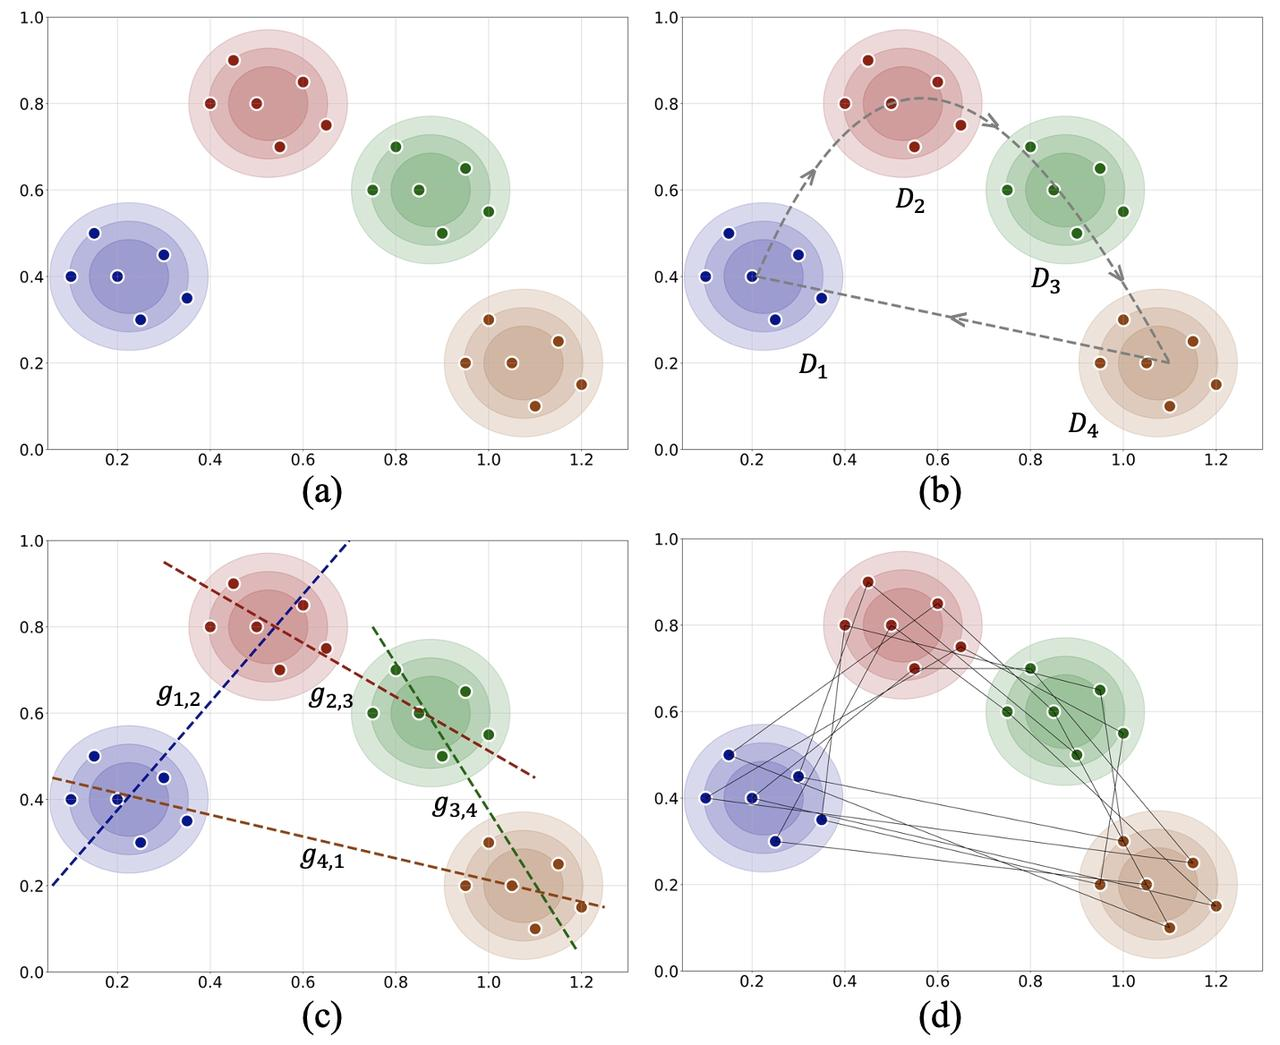
\includegraphics[width=0.9\textwidth]{figs/fig1.jpeg}
    \caption{方法整体流程图}
    \label{fig1}
\end{figure}
\\\hspace*{2em}图(a)中通过无监督聚类算法将原始特征空间划分为多个具有相近样本的特征子空间;图(b)中考虑了两维特征空间的情况对TSP问题进行求解,得到子空间插值排序方案;图(c)对相邻排序的子空间之间进行线性拟合;图(d)根据线性拟合的结果,通过多阶段最小权匹配算法求得相邻子空间之间的样本插值匹配策略并进行插值,合成误差较小的样本。

\section{特征子空间的划分}
在RSIS方法中,首先需要对原始数据集进行聚类,本文提出了一种无监督聚类算法,该方法可以将特征空间划分为多个等量样本的子空间,该算法分为两个阶段,迭代聚类阶段以及K近邻优化阶段。
\subsection{层次聚类}
迭代层次聚类过程的设计主要基于贪心策略的思想,通过多次循环迭代进行聚合聚类的无监督算法, 需要先给定超参数$k$,超参数$k$的直观解释是原始特征空间划分的子空间的数量。
\\\hspace*{2em}在首次迭代阶段,给定一个样本特征的有序集合$C_1=\left\{\boldsymbol{c}_i \right\}_{i=1}^n=\left\{\boldsymbol{x}_i \right\}_{i=1}^n$
,其中$\boldsymbol{c}_i$是集合$C_1$中的第$i$个元素。计算可得$C_1$中距离最近的两个元素$\boldsymbol{c}_p$和$\boldsymbol{c}_q$,其中
$p,q = \underset{\substack{p, q: p \neq q}}{\arg\min} \;\text{dist}(\boldsymbol{c}_p, \boldsymbol{c}_q)$
。随后,定义$D_{1}=\{\boldsymbol{c}_p,\boldsymbol{c}_q\},$作为第一个簇,根据公式\eqref{equ1}计算其簇心:

\begin{equation} \label{equ1}
	\bar{\boldsymbol{x}}^s = \frac{\sum_{\boldsymbol{x}^s \in D_s} \boldsymbol{x}^s}{\text{num}(D_s)}, 
\end{equation}
其中,$\text{num}(D_s)$是集合$D_s$中元素的数量。在首次迭代的最后,将$\boldsymbol{c}_p$和$\boldsymbol{c}_q$从$C_1$中剔除,并将集合$D_1$的簇心添加到$C_1$中作为下一次迭代的初始集合,即$C_{2}=\{\boldsymbol{c}_i \in C_{1} | i \neq p, q\} \cup \{\bar{\boldsymbol{x}}^1\}$.
\\\hspace*{2em}在随后的迭代过程中,都需要对于集合$C_t$求得最小距离的两个元素$\boldsymbol{c}_p,\boldsymbol{c}_q$。对于$\boldsymbol{c}_p$和$\boldsymbol{c}_q$分为三种情况进行讨论:$\boldsymbol{c}_p$和$\boldsymbol{c}_q$都是样本;一个是样本,另一个是簇心;两个都是簇心。
\\\hspace*{2em}在 \( \boldsymbol{c}_p, \boldsymbol{c}_q \) 都是原始样本的情况下,定义集合 \( D_s = \{ \boldsymbol{c}_p, \boldsymbol{c}_q  \} \) 生成新的簇并计算簇心 \( \bar{\boldsymbol{x}}^s \),将 \( \boldsymbol{c}_p, \boldsymbol{c}_q  \) 从集合 \( C_t \) 中剔除并且将 \( \bar{\boldsymbol{x}}^s \) 添加到集合 \( C_t \) 中,即 \( C_{t+1} = \{ \boldsymbol{c}_i \in C_t | i \neq p, q \} \cup \{ \bar{\boldsymbol{x}}^s \} \)。
\\\hspace*{2em}在\( \boldsymbol{c}_p\)是原始样本,\(\boldsymbol{c}_q:\bar{\boldsymbol{x}}^s\)是簇心的情况下,将\(\boldsymbol{c}_q\)添加到集合\(D_s\)中,并从\(C_t\)中将\(\boldsymbol{c}_q\)移除,根据公式\eqref{equ1}更新\(C_t\)中的簇心\(\bar{\boldsymbol{x}}^s\),即$C_{t+1}=\{\boldsymbol{c}_i \in C_{t} | i \neq p, q\} \cup \{{\bar{\boldsymbol{x}}^{s\prime}}\}$.
\\\hspace*{2em}若\( \boldsymbol{c}_p:\bar{\boldsymbol{x}}^s, \boldsymbol{c}_q:\bar{\boldsymbol{x}}^l \) 都是簇心,合并两个簇$D_s\leftarrow{D_s}{\;\cup\;}{D_l},$并且更新$D_s$的簇心,$C_{t+1}=\{\boldsymbol{c}_i \in C_{t} | i \neq p, q\} \cup \{{\bar{\boldsymbol{x}}^{s\prime}}\}$。
\\\hspace*{2em}每次迭代结束后,如果 \( \text{num}\left(D_s\right) \geq \left\lceil n/{k} \right\rceil \),则将 \( \bar{\boldsymbol{x}}^s \) 从 \( C_{t+1} \) 中剔除,并且引入LOF离群点检测\cite{ref52}算法对集合 \( D_s \) 中的样本进行离群点检测,剔除掉多余的样本点 \( \left\{ \boldsymbol{x}_i \right\}_{i=\left\lceil {n}/{k} \right\rceil+1}^{\text{num}\left(D_s\right)} \),将$D_s^{\prime}$作为一个完整的簇不参与后续迭代.
最后将通过LOF算法检测出来的多余的样本点重新添加到集合$C_{t+1}$中。当$C_{t+1}=\emptyset$则停止迭代。迭代聚类的直观过程可以参考图\ref{fig2}。

\begin{figure}[htbp]
    \centering
    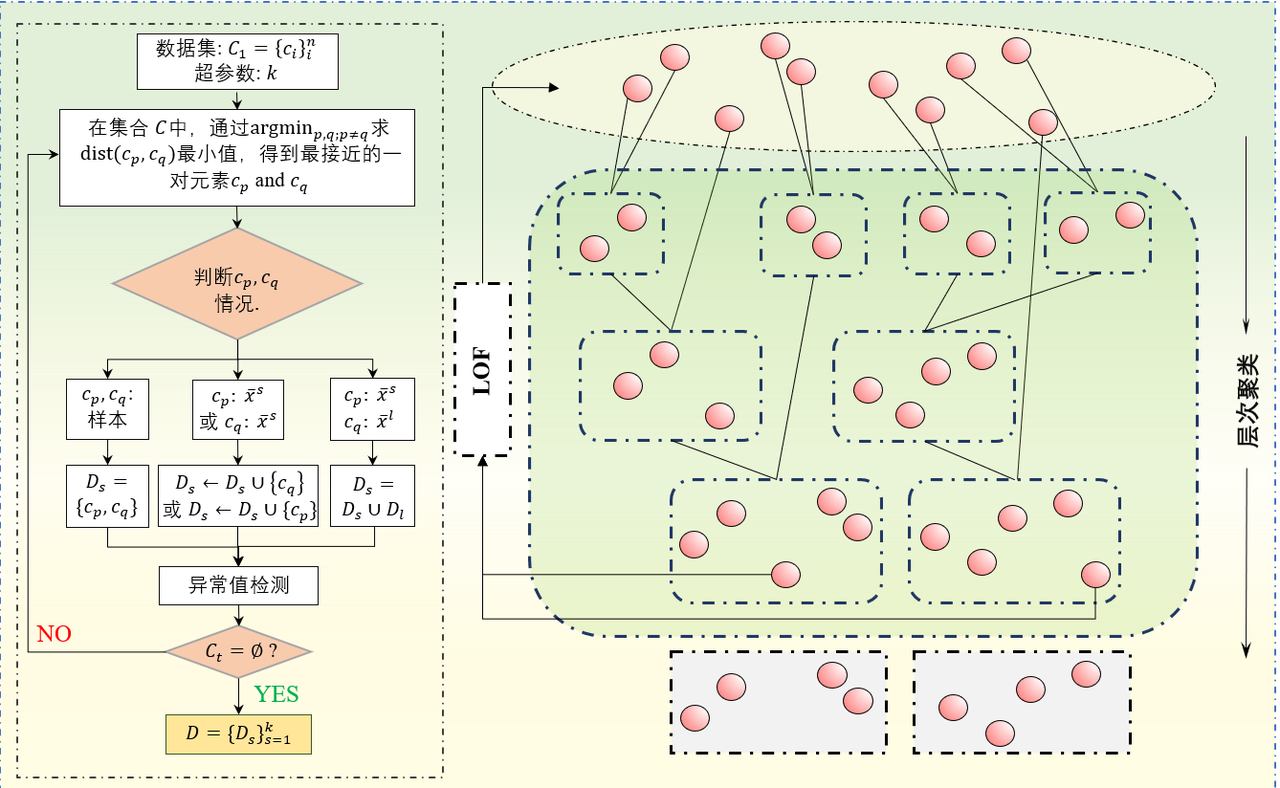
\includegraphics[width=1\textwidth]{figs/fig2.png}
    \caption{RSIS的层次聚类过程}
    \label{fig2}
\end{figure}

该迭代过程能够将原始数据集划分为 \(k-1\) 个子集,每个子集包含相等数量的样本以及一个额外的子集,该子集最多包含 \(\left\lceil n/k \right\rceil\) 个样本。形式上,本文定义
\(D=\cup_{s=1}^k D_s,\;  D_s=\{\boldsymbol{x}_i\}_{i=1}^l\),其中\(1 \leq l \leq \left\lceil {n/k} \right\rceil\)。
此外,RSIS 的迭代聚类过程将原始特征空间划分为 \(k\) 个特征子空间,表示为\(\mathcal{X} = \cup_{s=1}^{k} \mathcal{X}_s\)。迭代聚类具体过程详见算法\ref{a1}.
\\\hspace*{2em}在迭代的层次聚类过程中,需要计算得到集合中两个最接近的元素。这一步骤可以通过使用K-d树方法来进行优化。构建一个K-d树的时间复杂度通常为 \(O(n\log{n})\),而在K-d树中删除或添加一个点以及找到两个最近元素的平均时间复杂度为 \(O(\log{n})\)。然而,随着迭代的进行,样本大小会逐渐减少,因此实际的搜索时间会略有下降。在不考虑LOF离群点检测将簇中多余的样本重新放回数据集的情况下,那么迭代的总次数是 \(n\) 次。如果每次迭代都不重新构建K-d树,并且在现有的K-d树上进行查询和更新操作效率很高,那么整体的时间复杂度实际上会接近 \(O(n\log{n})\)。

\begin{algorithm}[!h]
    \caption{RSIS层次聚类}
    \label{a1}
    \renewcommand{\algorithmicrequire}{\textbf{Input:}}
    \renewcommand{\algorithmicensure}{\textbf{Output:}}
    \begin{algorithmic}[1]
        \REQUIRE 样本特征数据集$C$;超参数$k$  %%input
        \ENSURE $D=\{D_s\}_{s=1}^k$    %%output
        \WHILE{$C\neq{\emptyset}$}
            \STATE{计算得到特征空间中距离最近的两个元素$\boldsymbol{c}_p, \boldsymbol{c}_q$}
            \STATE{分为三种情况进行讨论:}
            \STATE{\qquad{}如果$\boldsymbol{c}_p, \boldsymbol{c}_q$都是样本}
                \STATE{\qquad{}\qquad{}定义新的簇$D_s=\{\boldsymbol{c}_p,\boldsymbol{c}_q\}$}
                \STATE{\qquad{}\qquad{}}计算$D_s$的簇心并添加到集合$C_t$中
                \STATE{\qquad{}\qquad{}将$\boldsymbol{c}_p, \boldsymbol{c}_q$从集合$C_t$中移除}
            \STATE{\qquad{}如果$\boldsymbol{c}_p$是原始样本,\(\boldsymbol{c}_q:\bar{\boldsymbol{x}}^s\)}
                \STATE{\qquad{}\qquad{}$D_s\leftarrow{D_s}\;{\cup}\;\{{\boldsymbol{c}}_q\}$}
                \STATE{\qquad{}\qquad{}在集合$C_t$中更新$D_s$的簇心}
                \STATE{\qquad{}\qquad{}将$\boldsymbol{c}_p$从集合$C_t$中移除}
            \STATE{\qquad{}如果\(\boldsymbol{c}_p:\bar{\boldsymbol{x}}^s\)和\(\boldsymbol{c}_q:\bar{\boldsymbol{x}}^l\)都是簇心}
                \STATE{\qquad{}\qquad{}$D_s\leftarrow{D_s}\;{\cup}\;D_l$}
                \STATE{\qquad{}\qquad{}在集合$C_t$中更新$D_s$的簇心}
                \STATE{\qquad{}\qquad{}将$\boldsymbol{c}_p$,$\boldsymbol{c}_p$从集合$C_t$中移除}
            \STATE{如果$\text{num}(D_s)\;\ge\;\left\lceil n/k\right\rceil$}
                \STATE{\qquad{}将$\bar{\boldsymbol{x}}^s$从集合$C_t$中移除}
                \STATE{\qquad{}利用LOF算法检测并剔除$D_s$中多余的样本}
                \STATE{\qquad{}将$\{\boldsymbol{x}^s_i\}_{i=\left\lceil n/k\right\rceil+1}^{\text{num}(D_s)}$添加至集合$C_t$中}
                \STATE{\qquad{}$D\;\leftarrow\;D\;{\cup}\;D_s$}
        \ENDWHILE

    \end{algorithmic}
\end{algorithm}
\newpage

\subsection{K近邻优化}
RSIS层次聚类过程基于贪心策略的思想,这种算法的设计在后期的迭代中可能会产生不合理的结果,从而影响整体的聚类效果。因此,本文引入了K最近邻(KNN)算法对上一阶段得到的聚类结果进行微调和优化。这种KNN的优化可能会影响每个簇中样本数量的平衡,但它将显著提高聚类的效果。
\\\hspace*{2em}初始聚类阶段完成后,RSIS的层次聚类阶段为每个样本分配一个标签,表示其所属的簇。在KNN优化阶段,会对每个样本计算其在特征空间中的$\left\lceil n/k\right\rceil$个最近邻的样本。随后,更新每个样本的簇标签,以反映其近邻样本中最频繁出现的簇标签。这一过程可能会导致一些样本的簇发生变化,从而引起每个簇内样本数量发生波动。有可能导致样本分布较为分散的簇被吸收至其他簇中,进而消失。然而,此优化过程确保了大多数簇的样本数量保持近似相等,并且显著提升了聚类的效果。通过将层次聚类过程与KNN优化相结合,可以得到最终的聚类结果$\{D_s\}_{s=1}^{k\prime}$,
其中,$k^{\prime}$表示示经过KNN优化后簇的数量。这种优化确保了簇间样本数量的均匀性,并且显著提升了聚类的总体质量(见图\ref{fig3})。

\begin{figure}[htbp]
    \centering
    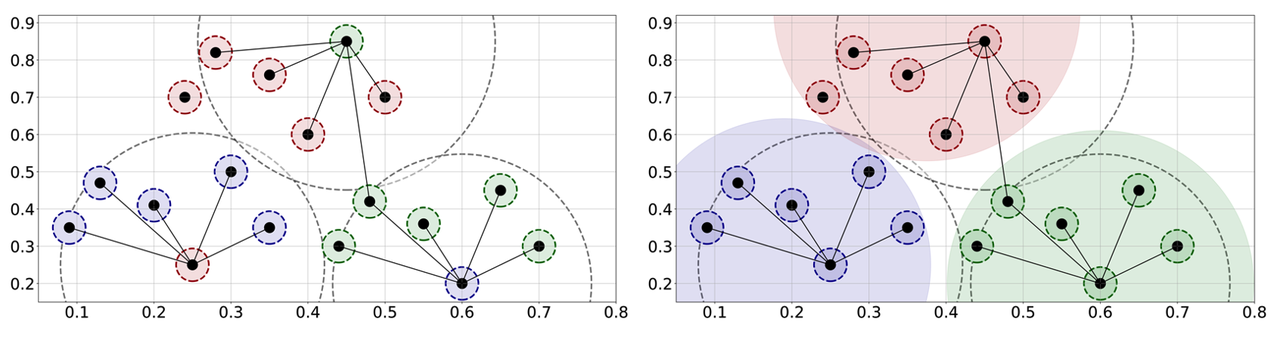
\includegraphics[width=1.0\textwidth]{figs/fig3.png}
    \caption{K近邻优化}
    \label{fig3}
\end{figure}

\section{子空间插值路径排序}
通过对原始数据进行聚类可以得到多个子集,每个子集对应不同的特征子空间。RSIS方法是对两个相邻的子空间之间的样本进行插值合成数据,该部分主要针对多个子空间插值路径排序的设计进行分析。
\\\hspace*{2em}插值路径的设计思想是从一个子空间出发,经过一次所有的子空间并最终返回起始点,目标是最小化总路径距离。可以转换为旅行商问题(TSP)进行求解,将该问题表示为一个加权图,其中每个子空间样本的簇心可以表示为顶点,簇心之间的直线路径可以表示为加权图的边,路径的距离可以表示为边的权重。设定目标函数:

\begin{equation} \label{equ2}
    \min{\sum\limits_{i=1}^{k'-1}\text{dist}(\boldsymbol{\bar{x}}^i,\boldsymbol{\bar{x}}^{i+1})}+\text{dist}(\boldsymbol{\bar{x}}^{k'},\boldsymbol{\bar{x}}^1). 
\end{equation}

旅行商问题是组合优化和理论计算机科学中的一个经典问题,也是一个典型的NP-hard问题,这意味着没有已知的多项式时间复杂度算法可以解决所有TSP实例,随着特征图顶点数量的增加,求解问题所需的时间和资源以指数级增长。
\\\hspace*{2em}在实际应用中,TSP被用来解决物流、规划、芯片制造等领域的问题\cite{ref53,ref54,ref55,ref56,ref57,ref58,ref59},但是直接解决TSP是非常复杂的,许多研究设计了多种启发式算法和近似算法来找到足够好的解\cite{ref60,ref61,ref62,ref63,ref64,ref65},虽然这些解不一定是最优的,这些方法通过不同的策略在可接受的时间内寻找到一个近似最短路径。
\\\hspace*{2em}为了保证能在可接受的时间内得到足够好的解决方案,本文首先使用贪婪算法快速找到一个初始解,然后用3-opt方法来优化并得到最终解。最终可以得到一个排序好的集合$D_\text{sorted}=\{D_{(s)}\}_{s=1}^{k'}$(如图\ref{fig4})。对应地,形式上定义排序好的特征子空间$\mathcal{X}_{\text{sorted}} = \cup_{s=1}^{k'} \mathcal{X}_{(s)}$。在后续的研究中,将序号相邻的两个子集所对应的子空间定义为相邻的特征子空间。
\begin{figure}[htbp]
    \centering
    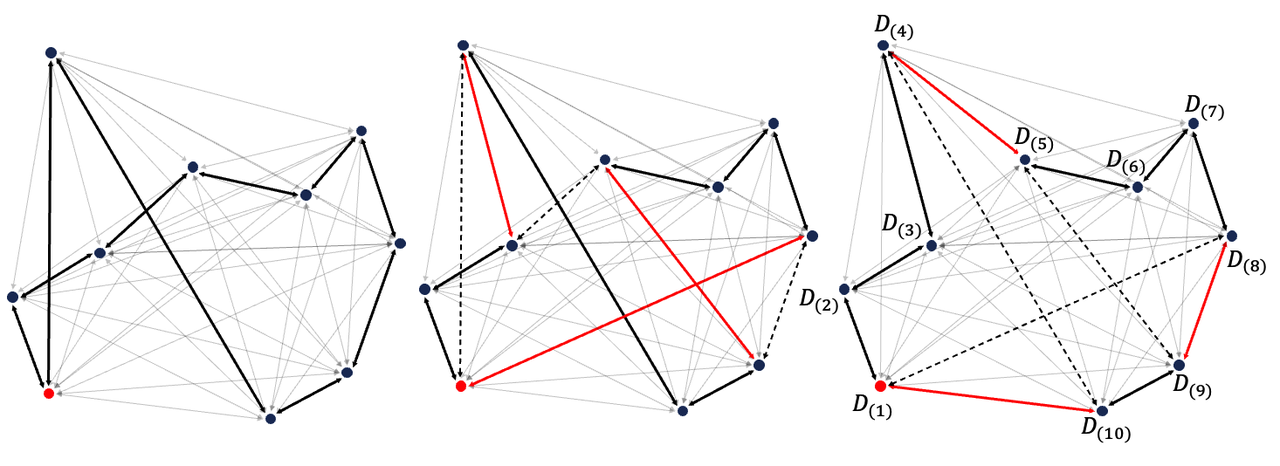
\includegraphics[width=1.0\textwidth]{figs/fig4.png}
    \caption{贪心算法结合3-opt对TSP问题求解}
    \label{fig4}
\end{figure}
\newpage
以上是针对多维度特征空间的研究,若特征空间是一维的,考虑到一维空间的特殊性,插值路径的设计依旧要求经过一次所有的子空间,但不需要重新回到起点,可以直接使用贪心策略进行求解,在一维情况下,这种方法得到的解一定是最优解。首先,定义插值路径的起点子空间:
\begin{equation} \label{equ3}
    D_{(1)}=\argmin_{\substack{D_{(s)}\in D_{\text{sorted}}}}\text{dist}({\bar{x}}^s,{x}_0),    
\end{equation}
其中,$x_o$是特征集合的最小值。对于后续簇的定义如下:
\begin{equation} \label{equ4}
    D_{(d)} = \argmin_{\substack{D_{(s)} \in D_{\text{sorted}}; \\ D_{(s)} \neq D_{(1)}, \ldots, D_{(d-1)}}}\text{dist}\left(\bar{x}^s, \bar{x}^{s-1}\right).   
\end{equation}
\\\hspace*{2em}除非另有特别说明,本文后续的研究主要集中在多维特征空间情况下进行探讨。

\section{相邻子空间线性回归拟合}

给定含噪数据集$D=\{\boldsymbol{x}_i,y_i\}_{i=1}^n$,其中$\boldsymbol{x}_i\in \mathcal{X}=\mathbb{R}^d$,以及$y_i\in\mathcal{Y}=\mathbb{R}$。考虑关系式$\dot{y}_i=f(\dot{\boldsymbol{x}}_i)$,其中$\dot{\boldsymbol{x}}_i$,$\dot{y}_i$分别是$\boldsymbol{x}_i$,$y_i$的去噪真实值。在RSIS方法中,假设函数$f(\cdot)$是连续的,可得:
\begin{equation} \label{equ5}
\dot{y}_i+\varepsilon_{i,y}=f(\dot{\boldsymbol{x}}_i+\boldsymbol{\varepsilon}_{i,x})+\varepsilon_i,
\end{equation}
其中,$\boldsymbol{\varepsilon}_{i,x}$,$\varepsilon_{i,y}$分为$\dot{\boldsymbol{x}}_i$,$\dot{y}_i$所含的噪音,$\varepsilon_i$为等式的误差项。等式\eqref{equ5}可以转化为:
\begin{equation} \label{equ6}
    y_i=f(\boldsymbol{x}_i)+\varepsilon_i.     
\end{equation}
\hspace*{2em}通过上述聚类以及排序方法,可以将原始数据集划分为多个有序的子集$D_\text{sorted}=\{D_{(s)}\}_{s=1}^{k'}$,其中$D_{(s)}=\{ \boldsymbol{x}_i^s,y_i^s \}_{i=1}^{\text{num}(D_{(s)})}$,
并且特征空间可以划分为多个有序的子空间$\mathcal{X}=\cup_{s=1}^{k^\prime}\mathcal{X}_{(s)}$。
对于两个相邻的特征子空间,由于假设函数$f(\cdot)$是连续的,因此函数$f(\cdot)$可以被近似拟合为一个线性函数$g(\cdot)$,公式\eqref{equ6}可以转化为:
\begin{equation} \label{equ7}
    y_i^{s,s+1}=g_{s,s+1}(\boldsymbol{x}_i^{s,s+1})+\varepsilon_i+\varepsilon_i^\prime,
\end{equation}
其中,$g(\cdot)$以及$\varepsilon_i^\prime$分别表示子空间$\mathcal{X}^{(s)}$和$\mathcal{X}^{(s+1)}$中的线性拟合函数以及线性拟合误差,$\{\boldsymbol{x}_i^{s,s+1},y_i^{s,s+1}\}\in D_s\cup D_{s+1}$。如果两个子空间的距离足够近并且测度趋向于零,则线性拟合误差$\varepsilon_i^\prime\rightarrow0$。
\\\hspace*{2em}对相邻的两个子空间进行线性拟合,可以考虑使用Ordinary Least Squares (OLS)、Lasso,或者局部线性回归等方法\cite{ref66,ref67,ref68}。然而,在假设$f(\cdot)$是一个连续函数的前提下,仅基于两个子空间的样本进行线性拟合,并没有充分考虑到全局信息。因此,本文引入了软参数共享机制\cite{ref3,ref69,ref70,ref71,ref72},同时估计多个子空间之间的线性拟合函数,并且在损失函数中添加了$L_1$正则项。这种方法确保了每个线性函数$\hat{g}_{s,s+1}(\cdot)$的估计都融入了全局信息。
\begin{equation} \label{equ8}
    \begin{aligned}
        L(\boldsymbol{\beta}) = & \sum\limits_{s=2}^{k^\prime-1}\left(L_2(\boldsymbol{\beta}^{s,s+1}) + \frac{\lambda}{\text{dist}(\overline{\boldsymbol{x}}^{s}, \overline{\boldsymbol{x}}^{s-1}) + 1}L_1(\boldsymbol{\beta}^{s,s+1}, \boldsymbol{\beta}^{s-1,s}) \right) \\
        & + L_2(\boldsymbol{\beta}^{1,2}) + L_2(\boldsymbol{\beta}^{k^\prime,1})\\
        &+ \frac{\lambda}{\text{dist}(\overline{\boldsymbol{x}}^{k^\prime}, \overline{\boldsymbol{x}}^{1}) + 1}(L_1(\boldsymbol{\beta}^{1,2}, \boldsymbol{\beta}^{k^\prime,1})+L_1(\boldsymbol{\beta}^{k^\prime,1},
        \boldsymbol{\beta}^{k^\prime-1,k^\prime}))
    \end{aligned}
\end{equation}
其中,$$\boldsymbol{\beta}=\left(\boldsymbol{\beta}^{1,2},\boldsymbol{\beta}^{2,3},\ldots,\boldsymbol{\beta}^{k^\prime-1,k^\prime},\boldsymbol{\beta}^{k^\prime,1}\right)^\prime,$$ 
$$L_2(\boldsymbol{\beta}^{p,q})=\left\|\boldsymbol{y}^{p, q}-\boldsymbol{X}^{p, q} \boldsymbol{\beta}^{p, q}\right\|_{2}^{2},$$ $$L_1(\boldsymbol{\beta}^{q,r},\boldsymbol{\beta}^{p,q})=\|\boldsymbol{\beta}^{q,r}-\boldsymbol{\beta}^{p,q}\|_1.$$ $\dfrac{\lambda}{\text{dist}(\overline{\boldsymbol{x}}^{s},\overline{\boldsymbol{x}}^{s-1})+1}$
作为正则项参数,可以自适应的根据子空间之间的距离进行调整。在后文的实验中,本文设置$\lambda=1$。本文在引理\ref{lemma1}以及引理\ref{lemma2}的基础上,通过定理\ref{thm1}证明了公式\eqref{equ8}是凸函数,这确保了该函数局部最优解就是全局最优解。
\begin{lemma}
    \label{lemma1}
	对于函数$f(\boldsymbol{\beta})=\|\boldsymbol{y}-\boldsymbol{X}\boldsymbol{\beta}\|_2^2$,
    其中$\boldsymbol{y}\in\mathbb{R}^{n\times1}$,$\boldsymbol{X}\in\mathbb{R}^{n\times d}$,$\boldsymbol{\beta}\in\mathbb{R}^{d\times1}$。对于$\forall\omega\in[0,1]$,以及$\forall\boldsymbol{\beta}_1,\boldsymbol{\beta}_2\in\mathbb{R}^{d\times1}$可得:
    \begin{equation}
        f(\omega\boldsymbol{\beta}_1+(1-\omega)\boldsymbol{\beta}_2)\le\omega f(\boldsymbol{\beta}_1)+(1-\omega)f(\boldsymbol{\beta}_2).
    \end{equation}
\end{lemma}
\noindent \textbf{证明(引理\ref{lemma1})}:考虑函数$f(\boldsymbol{\beta})=\|\boldsymbol{y}-\boldsymbol{X}\boldsymbol{\beta}\|_2^2$
,其中$\|\boldsymbol{y}-\boldsymbol{X}\boldsymbol{\beta}\|_2$表示$\boldsymbol{y}-\boldsymbol{X}\boldsymbol{\beta}$的$L_2$正则项。对于$\forall\omega\in[0,1]$以及$\forall\boldsymbol{\beta}_1,\boldsymbol{\beta}_2\in\mathbb{R}^{d\times1}$,可得:
$$
\begin{aligned}
    &\qquad f(\omega\boldsymbol{\beta}_1+(1-\omega)\boldsymbol{\beta_2})- \omega f(\boldsymbol{\beta_1})-(1-\omega)f(\boldsymbol{\beta_2}) \\
    &=||y-X(\omega\boldsymbol{\beta}_1+(1-\omega)\boldsymbol{\beta}_2)||_2^2-\omega||y-X\boldsymbol{\beta}_1||_2^2-(1-\omega)||y-X\boldsymbol{\beta}_2||_2^2 \\
    &=||\omega y+(1-\omega)y-X(\omega\boldsymbol{\beta}_1+(1-\omega)\boldsymbol{\beta}_2)||_2^2-\omega||y-X\boldsymbol{\beta}_1||_2^2-(1-\omega)||y-X\boldsymbol{\beta}_2||_2^2 \\
    &=||\omega(y-X\boldsymbol{\beta}_1)+(1-\omega)(y-X\boldsymbol{\beta}_2)||_2^2-\omega||y-X\boldsymbol{\beta}_1||_2^2-(1-\omega)||y-X\boldsymbol{\beta}_2||_2^2 \\
    &=\omega^2||y-X\boldsymbol{\beta}_1||_2^2+(1-\omega)^2||y-X\boldsymbol{\beta}_2||_2^2 +2\omega(1-\omega)(y-X\boldsymbol{\beta}_1)^\prime(y-X\boldsymbol{\beta}_2)\\
    &\quad{}-\omega||y-X\boldsymbol{\beta}_1||_2^2-(1-\omega)||y-X\boldsymbol{\beta}_2||_2^2 \\
    &=\omega^2||y-X\boldsymbol{\beta}_1||_2^2+(1-2\omega+\omega^2)||y-X\boldsymbol{\beta}_2||_2^2 +(2\omega-2\omega^2)(y-X\boldsymbol{\beta}_1)^\prime(y-X\boldsymbol{\beta}_2)\\
    &\quad{}-\omega||y-X\boldsymbol{\beta}_1||_2^2-(1-\omega)||y-X\boldsymbol{\beta}_2||_2^2 \\
    &=\omega^2\left(||y-X\boldsymbol{\beta}_1||_2^2 - 2(y-X\boldsymbol{\beta}_1)^\prime(y-X\boldsymbol{\beta}_2)+||y-X\boldsymbol{\beta}_2||_2^2 \right)+(1-2\omega)||y-X\boldsymbol{\beta}_2||_2^2\\
    &\quad{}+2\omega(y-X\boldsymbol{\beta}_1)^\prime(y-X\boldsymbol{\beta}_2)-\omega||y-X\boldsymbol{\beta}_1||_2^2-(1-\omega)||y-X\boldsymbol{\beta}_2||_2^2 \\
    &=\omega^2||(y-X\boldsymbol{\beta}_1)-(y-X\boldsymbol{\beta}_2)||_2^2+2\omega(y-X\boldsymbol{\beta}_1)^\prime(y-X\boldsymbol{\beta}_2)-\omega||y-X\boldsymbol{\beta}_1||_2^2\\
    &\quad{}-\omega||y-X\boldsymbol{\beta}_2||_2^2 \\
    &=\omega^2||(y-X\boldsymbol{\beta}_1)-(y-X\boldsymbol{\beta}_2)||_2^2-\omega||(y-X\boldsymbol{\beta}_1)-(y-X\boldsymbol{\beta}_2)||_2^2 \\
    &=\omega(\omega-1)||(y-X\boldsymbol{\beta}_1)-(y-X\boldsymbol{\beta}_2)||_2^2 \le0.
\end{aligned}
$$
通过不等式$$f(\omega\boldsymbol{\beta}_1+(1-\omega)\boldsymbol{\beta}_2)- \omega f(\boldsymbol{\beta}_1)-(1-\omega)f(\boldsymbol{\beta}_2)\le0,$$
推导可得凸性条件:$$
    f(\omega\boldsymbol{\beta}_1+(1-\omega)\boldsymbol{\beta}_2)\le \omega f(\boldsymbol{\beta}_1)+(1-\omega)f(\boldsymbol{\beta}_2).$$

\begin{lemma} \label{lemma2}
	对于函数$f(\boldsymbol{\beta})=\|\boldsymbol{\beta}^1-\boldsymbol{\beta}^2\|_1$,其中$\boldsymbol{\beta}^1,\boldsymbol{\beta}^2\in\mathbb{R}^{d\times1}$,$\boldsymbol{\beta}=((\boldsymbol{\beta}^1)^\prime,(\boldsymbol{\beta}^2)^\prime)^\prime$。对于$\forall\omega\in[0,1]$以及$\forall\boldsymbol{\beta}_1,\boldsymbol{\beta}_2\in\mathbb{R}^{2d\times1}$,可得:
	\begin{equation}
        f(\omega\boldsymbol{\beta}_1+(1-\omega)\boldsymbol{\beta}_2)\le\omega f(\boldsymbol{\beta}_1)+(1-\omega)f(\boldsymbol{\beta}_2).
    \end{equation}
\end{lemma}

\noindent \textbf{证明(引理\ref{lemma2})}:考虑到$f(\boldsymbol{\beta})$关于$L_1$范数的线性结构:
$$\begin{aligned}
    f(\omega\boldsymbol{\beta}_1+(1-\omega)\boldsymbol{\beta}_2)&=||(\omega\boldsymbol{\beta}_1^1+(1-\omega)\boldsymbol{\beta}_2^1)-(\omega\boldsymbol{\beta}_1^2+(1-\omega)\boldsymbol{\beta}_2^2)||_1 \\
    &= ||\omega(\boldsymbol{\beta}_1^1-\boldsymbol{\beta}_1^2)+(1-\omega)(\boldsymbol{\beta}_2^1-\boldsymbol{\beta}_2^2)||_1 \\
    &\le \omega||\boldsymbol{\beta}_1^1-\boldsymbol{\beta}_1^2||_1+(1-\omega)||\boldsymbol{\beta}_2^1-\boldsymbol{\beta}_2^2||_1 \\
    &= \omega f(\boldsymbol{\beta}_1)+(1-\omega)f(\boldsymbol{\beta}_2)
    \end{aligned}$$

\begin{theorem}[由引理\ref{lemma1},引理\ref{lemma2}导出的不等式] \label{thm1}
	根据等式\eqref{equ8},对于$\forall\omega\in[0,1]$,以及$\forall\boldsymbol{\beta}_1,\boldsymbol{\beta}_2\in\mathbb{R}^{d\times k^\prime}$,可得:
    \begin{equation}
        L(\omega\boldsymbol{\beta}_1+(1-\omega)\boldsymbol{\beta}_2)\le\omega L(\boldsymbol{\beta}_1)+(1-\omega)L(\boldsymbol{\beta}_2).
    \end{equation}
\end{theorem}

\noindent \textbf{证明(定理\ref{thm1})}:令$$\lambda_{p,q}=\dfrac{\lambda}{\text{dist}(\overline{\boldsymbol{x}}^{p},\overline{\boldsymbol{x}}^{q})+1},\;L(\boldsymbol{\beta})=\gamma_1(\boldsymbol{\beta})+\gamma_2(\boldsymbol{\beta}),$$
其中$$\gamma_1(\boldsymbol{\beta})=\sum\limits_{s=2}^{k^\prime-1}\lambda_{s,s-1}L_1(\boldsymbol{\beta}^{s,s+1},\boldsymbol{\beta}^{s-1,s}) +\lambda_{k^\prime,1}L_1(\boldsymbol{\beta}^{1,2},\boldsymbol{\beta}^{k^\prime,1})+\lambda_{k^\prime-1,k^\prime}L_1(\boldsymbol{\beta}^{k^\prime,1},
\boldsymbol{\beta}^{k^\prime-1,k^\prime}),$$
$$\gamma_2(\boldsymbol{\beta})=\sum\limits_{s=1}^{k^\prime-1}L_2(\boldsymbol{\beta}^{s,s+1})+L_2(\boldsymbol{\beta}^{k^\prime,1}),$$
可得:$$L(\omega\boldsymbol{\beta}_1+(1-\omega)\boldsymbol{\beta}_2)=\gamma_1(\omega\boldsymbol{\beta}_1+(1-\omega)\boldsymbol{\beta}_2)+\gamma_2(\omega\boldsymbol{\beta}_1+(1-\omega)\boldsymbol{\beta}_2).$$
基于引理\ref{lemma1}和引理\ref{lemma2}可得:
$$L_1(\omega\boldsymbol{\beta}^{q,r}_1+(1-\omega)\boldsymbol{\beta}^{q,r}_2,\omega\boldsymbol{\beta}^{p,q}_1+(1-\omega)\boldsymbol{\beta}^{p,q}_2)\le\omega L_1(\boldsymbol{\beta}^{q,r}_1,\boldsymbol{\beta}^{p,q}_1)+(1-\omega)L_1(\boldsymbol{\beta}_2^{q,r},\boldsymbol{\beta}^{p,q}_2),$$
以及$$L_2(\omega\boldsymbol{\beta}^{p,q}_1+(1-\omega)\boldsymbol{\beta}^{p,q}_2)\le\omega L_2(\boldsymbol{\beta}^{p,q}_1)+(1-\omega)L_2(\boldsymbol{\beta}^{p,q}_2).$$
进一步地:
$$\begin{aligned}
    \gamma_1(\omega\boldsymbol{\beta}_1+(1-\omega)\boldsymbol{\beta}_2)
    &\le \sum\limits_{s=2}^{k^\prime-1}\lambda_{s,s-1}(\omega L_1(\boldsymbol{\beta}^{s,s+1}_1,\boldsymbol{\beta}^{s-1,s}_1)+(1-\omega)L_1(\boldsymbol{\beta}_2^{s,s+1},\boldsymbol{\beta}^{s-1,s}_2))  \\ &+\lambda_{k^\prime,1}(\omega L_1(\boldsymbol{\beta}^{1,2}_1,\boldsymbol{\beta}^{k^\prime,1}_1)+(1-\omega)L_1(\boldsymbol{\beta}_2^{1,2},\boldsymbol{\beta}^{k^\prime,1}_2)) \\
    &=\omega\gamma_1(\boldsymbol{\beta}_1)+(1-\omega)\gamma_1(\boldsymbol{\beta}_2).
    \end{aligned}$$
$$\begin{aligned}
    \gamma_2(\omega\boldsymbol{\beta}_1+(1-\omega)\boldsymbol{\beta}_2)
    &\le\sum\limits_{s=1}^{k^\prime-1}(\omega L_2(\boldsymbol{\beta}^{s,s+1}_1)+(1-\omega)L_2(\boldsymbol{\beta}^{s,s+1}_2))+\omega L_2(\boldsymbol{\beta}^{k^\prime,1}_1)\\
    &+(1-\omega)L_2(\boldsymbol{\beta}^{k^\prime,1}_2) \\
    &=\omega\gamma_2(\boldsymbol{\beta}_1)+(1-\omega)\gamma_2(\boldsymbol{\beta}_2).
    \end{aligned}$$
因此,由上可得:
$$\begin{aligned} L(\omega\boldsymbol{\beta}_1+(1-\omega)\boldsymbol{\beta}_2)
    &=\gamma_1(\omega\boldsymbol{\beta}_1+(1-\omega)\boldsymbol{\beta}_2)+\gamma_2(\omega\boldsymbol{\beta}_1+(1-\omega)\boldsymbol{\beta}_2) \\
    &\le \omega\gamma_1(\boldsymbol{\beta}_1)+(1-\omega)\gamma_1(\boldsymbol{\beta}_2)+\omega\gamma_2(\boldsymbol{\beta}_1)+(1-\omega)\gamma_2(\boldsymbol{\beta}_2) \\
    &=\omega L(\boldsymbol{\beta}_1)+(1-\omega)L(\boldsymbol {\beta}_2)
    . \end{aligned}$$

\section{多阶段最小权匹配}
接下来需要对相邻的两个子空间的样本进行等距线性插值合成新的样本,插值的过程是在两个样本之中进行的,RSIS方法生成的数据要充分考虑到所有的样本信息,插值规则设计如下:
\\\hspace*{2em}1.插值的两个样本应当来自不同的子空间;
\\\hspace*{2em}2.每个样本至少进行一次插值;
\\\hspace*{2em}3.插值总次数为$\max(\text{num}{(D_{(s)}),\text{num}(D_{(s+1)})})$;
\\\hspace*{2em}4.所有样本参与插值的次数必须是均匀的,即每个样本最多插值次数为$$\left\lceil \frac{\max(\text{num}{(D_{(s)}),\text{num}(D_{(s+1)})})}{\min(\text{num}{(D_{(s)}),\text{num}(D_{(s+1)})})}\right\rceil.$$
\\\hspace*{2em}由于数据集$D_{\text{sorted}}$包含未知噪音,通过插值合成的样本会受到原始样本噪音的影响也会包含噪音。在对两个相邻子空间进行线性插值时,插值匹配策略的选择需要考虑到合成的样本相比真实分布的误差。
不失一般性,假设$\text{num}(D_{(s)})=m,\text{num}(D_{(s+1)})=n,$,并且$n/2\le{m}\le{n}$。根据插值规则,共有$
C_{n-2k}^{2}\prod_{k=0}^{n-m-1} C_{m}^{n-m}(2m-n)!$种不同的插值匹配策略可供选择。如何快速选择一个较优的插值匹配策略是本文需要重点探讨的问题。
\\\hspace*{2em}同样不失一般性,假设特征空间的维度是一维的,定义公式\eqref{equ12}来量化两个原始样本之间进行线性且等距插值合成的样本的平均误差:

\begin{equation}\label{equ12}
\bar{S}(x^s,x^{s+1})=\frac{\int_{x^s}^{x^{s+1}}|f(x)-l(x)| dx}{|x^{s+1}-x^s|}, 
\end{equation}
其中,$l(x)$表示为经过$(x^s,y^s)$和$(x^{s+1},y^{s+1})$两个样本点的线性函数,$f(\cdot)$为$x$,$y$真实的函数关系。

\begin{theorem}\label{thm2}
	对于两个相邻的特征子空间$\mathcal{X}_{(s)}$,$\mathcal{X}_{(s+1)}$的样本$(x^s,y^s)\in{D}_{(s)}\;\text{和}\; (x^{s+1},y^{s+1})\in{D}_{(s+1)}$,考虑$y=f(x)+\varepsilon$。根据公式\eqref{equ7},假设线性拟合误差$\varepsilon^\prime\rightarrow0$,可得:
    \begin{equation}
        \mathbb{E}(\bar{S}(x^s,x^{s+1}))\;<\;\mathbb{E}(\frac{|\varepsilon^s|+|\varepsilon^{s+1}|}{2}).    
    \end{equation}
\end{theorem}
\noindent \textbf{证明(定理\ref{thm2})}:由于$\varepsilon^\prime\rightarrow0$,根据公式\eqref{equ7}:
$$y^{s,s+1}=g_{s,s+1}(x^{s,s+1})+\varepsilon.$$
代入公式\eqref{equ12},可转化为:
$$\bar{S}(x^s,x^{s+1})=\frac{\int_{x^s}^{x^{s+1}}|g(x)-l(x)| dx}{|x^{s+1}-x^s|}.$$
根据迭代期望定律(Law of Iterated Expectations,LIE):
$$\begin{aligned}
    \mathbb{E}(\bar{S}(x^s,x^{s+1}))&=\mathbb{E}(\bar{S}(x^s,x^{s+1})|\varepsilon^s\cdot\varepsilon^{s+1}<0)P(\varepsilon^s\cdot\varepsilon^{s+1}<0)\\
    &\quad\; +\mathbb{E}(\bar{S}(x^s,x^{s+1})|\varepsilon^s\cdot\varepsilon^{s+1}\ge0)P(\varepsilon^s\cdot\varepsilon^{s+1}\ge0).
    \end{aligned}$$
可以利用基础的几何面积计算来简化$\bar{S}(x^s,x^{s+1})$。
若$\varepsilon^s\cdot\varepsilon^{s+1}<0$,则$\exists{x'}\in(x^s,x^{s+1})$,
使得$g(x')=l(x')$。可得:
$$\mathbb{E}(\bar{S}(x^s,x^{s+1})|\varepsilon^s\cdot\varepsilon^{s+1}<0)=\frac{\mathbb{E}(|\varepsilon^s|)\cdot|x^s-x'|+\mathbb{E}(|\varepsilon^{s+1}|)\cdot|x^{s+1}-x'|}{2|x^{s+1}-x^s|}.$$
若$\varepsilon^s\cdot\varepsilon^{s+1}\ge0$,则有:
$$\begin{aligned}
    \mathbb{E}(\bar{S}(x^s,x^{s+1})|\varepsilon^s\cdot\varepsilon^{s+1}\ge0)&=\frac{\mathbb{E}(|\varepsilon^s|+|\varepsilon^{s+1}|)\cdot|x^{s+1}-x^{s}|}{2|x^{s+1}-x^s|}\\&=\frac{\mathbb{E}(|\varepsilon^s|+|\varepsilon^{s+1}|)}{2}.
    \end{aligned}$$
代入原等式,有:
$$\begin{aligned}
    \mathbb{E}({\bar{S}(x^{s}, x^{(s+1)})})&=
    \frac{{\mathbb{E}(|\varepsilon^s|)\cdot|x^s-x'|+\mathbb{E}(|\varepsilon^{s+1}|)\cdot|x^{s+1}-x'|}}{2|x^{s+1}-x^s|}P(\varepsilon^s\cdot\varepsilon^{s+1}<0)\\
    &\;\quad+\frac{\mathbb{E}(|\varepsilon^s|+|\varepsilon^{s+1}|)}{2}P(\varepsilon^s\cdot\varepsilon^{s+1}\ge0).
    \end{aligned}$$
由于$P(\varepsilon^s\cdot\varepsilon^{s+1}<0)+P(\varepsilon^s\cdot\varepsilon^{s+1}\ge0)=1$,并且:
$$\begin{aligned}
    \frac{{\mathbb{E}(|\varepsilon^s|)\cdot|x^s-x'|+\mathbb{E}(|\varepsilon^{s+1}|)\cdot|x^{s+1}-x'|}}{2|x^{s+1}-x^s|}&=
    \frac{{\mathbb{E}(|\varepsilon^s|)\cdot|\frac{x^s-x'}{x^{s+1}-x^s}|+\mathbb{E}(|\varepsilon^{s+1}|)\cdot|\frac{x^{s+1}-x'}{x^{s+1}-x^s}|}}{2}\\
    &<\frac{{\mathbb{E}(|\varepsilon^s|)+\mathbb{E}(|\varepsilon^{s+1}|)}}{2},
\end{aligned}$$
因此,得证:
$$\mathbb{E}(\bar{S}(x^s,x^{s+1}))<\mathbb{E}(\frac{|\varepsilon^s|+|\varepsilon^{s+1}|}{2}).$$
\newpage
通过定理\ref{thm2}可知,在线性拟合误差$\varepsilon_i^\prime\rightarrow0$的假设条件下,即使是面对噪音不同分布的情况,对任意两个子空间中的样本进行等距线性插值生成的样本均匀噪音的期望小于原始样本噪音的平均期望。
\begin{theorem}\label{thm3}
	与定理\ref{thm2}的场景下,令$y^s=f(x^s)+\varepsilon^s$,$y^{s+1}=f(x^{s+1})+\varepsilon^{s+1}$。假设线性拟合误差$\varepsilon^\prime\rightarrow0$,可得:
    \begin{equation}\label{equ14}
        \bar{
S}(x^s,x^{s+1})= \begin{cases} 
\dfrac{|\frac{\varepsilon^s}{\varepsilon^s-\varepsilon^{s+1}}|\cdot|\varepsilon^{s}|+|\frac{\varepsilon^{s+1}}{\varepsilon^s-\varepsilon^{s+1}}|\cdot|\varepsilon^{s+1}|}{2},\quad\varepsilon^s\cdot \varepsilon^{s+1}<0,
\\
\\
\dfrac{|\varepsilon^s|+|\varepsilon^{s+1}|}{2}, \qquad\qquad\qquad\qquad\;\;\;\;\varepsilon^s\cdot \varepsilon^{s+1}\ge0.
\end{cases}    
    \end{equation}
\end{theorem}

\noindent \textbf{证明(定理\ref{thm3})}:当$\varepsilon^s\cdot\varepsilon^{s+1}<0$时,$\exists x'\in(x^s,x^{s+1})$,使得
$g(x')=l(x')$。可得:
$$\begin{aligned}
    \bar{
    S}(x^s,x^{s+1})&=\frac{|\varepsilon^{s}|\cdot|x^{s}-x'|+|\varepsilon^{s+1}|\cdot|x^{s+1}-x'|}{2|x^s-x^{s+1}|}\\
    &=\frac{|\varepsilon^{s}|\cdot|\frac{x^s-x'}{x^{s}-x^{s+1}}|+|\varepsilon^{s+1}|\cdot|\frac{x^{s+1}-x'}{x^{s}-x^{s+1}}|}{2}.
    \end{aligned}$$
基于相似三角形性质,有:
$$|\frac{x^s-x'}{x^{s}-x^{s+1}}|=|\frac{\varepsilon^s}{\varepsilon^s-\varepsilon^{s+1}}|,$$
$$|\frac{x^{s+1}-x'}{x^{s}-x^{s+1}}|=|\frac{\varepsilon^{s+1}}{\varepsilon^s-\varepsilon^{s+1}}|.$$
代入原式:
$$\begin{aligned}
    \bar{
    S}(x^s,x^{s+1})&=
    \frac{|\frac{\varepsilon^s}{\varepsilon^s-\varepsilon^{s+1}}|\cdot |\varepsilon^{s}|+|\frac{\varepsilon^{s+1}}{\varepsilon^s-\varepsilon^{s+1}}|\cdot|\varepsilon^{s+1}|}{2}\\&<
    \frac{|\varepsilon^s|+|\varepsilon^{s+1}|}{2}.
    \end{aligned}$$
若当$\varepsilon^s\cdot\varepsilon^{s+1}\ge0$时:
$$\begin{aligned}
    \bar{
    S}(x^s,x^{s+1})&=\frac{(|\varepsilon^s|+|\varepsilon^{s+1}|)\cdot|x^{s+1}-x^{s}|}{2|x^{s+1}-x^{s}|}\\&=
    \frac{|\varepsilon^s|+|\varepsilon^{s+1}|}{2}.
    \end{aligned}$$
综上,得证。
\\\hspace*{2em}通过定理\ref{thm3}可以对公式\eqref{equ12}进行简化。可以利用子空间之间的线性拟合函数来估计样本误差,然后利用二分图最小权匹配方法根据误差信息确定匹配策略。在假设条件下,样本的噪声可以根据公式\eqref{equ7}估计得到:
\begin{equation}\label{equ15}
    \varepsilon_i^{s,s+1}=y_i^{s,s+1}-g_{s,s+1}(\boldsymbol{x}_i^{s,s+1}).    
\end{equation}
\hspace*{2em}随后可以将原始问题转换为最小权匹配问题求解。近些年来,最小权匹配问题在物流、网络设计、资源分配等领域有广泛应用\cite{ref73,ref74,ref75};也有部分研究将最小权匹配问题扩展到更复杂的网络中,例如动态网络或随机网络,研究如何在变化的环境中找到最优解\cite{ref76,ref77,ref78};对于那些计算上不可行求解精确结果的大型问题,一些研究可能会寻找能够快速得到近似解的算法\cite{ref79,ref80}。
\\\hspace*{2em}根据插值规则,需要对每个样本至少进行一次插值,并且约束了插值的总次数。经过K近邻优化后子空间之间的样本数量大多数情况并不是完全相等的,所以这不能视作一个最小权完美匹配问题。这个问题是一个加权匹配问题的变体,同时融合了平衡匹配和最小权匹配的特点,因为它需要最小化匹配的总权重,并且约束了样本匹配次数的均匀性。目前针对这种问题并没有一个现成的标准算法,因此需要对传统的最小权匹配问题进行改进以适应此目标场景。本文提出了一种启发式的多阶段的最小权匹配方法对该问题进行分析。需要注意的是,这种方法并不能保重所得结果是一个最优解,但是但它可以在极短的时间内得到一个合理的近似解。这种方法的优点在于它相对简单,并且对于大规模问题来说可以提供较好的效率,如果需要找到最优解,可能需要使用更复杂的优化方法,例如整数线性规划(ILP)来精确求解问题,但通常需要更多的计算资源和时间。
\\\hspace*{2em}依旧延续上文的假设,$\text{num}(D_{(s)})=m,\text{num}(D_{(s+1)})=n,\;n/2\le m\le n$。在这种场景下,$D_{(s)}$中的每个样本都需要进行一次或者两次的插值,因此将该问题分为两个阶段进行求解。
\\\hspace*{2em}给定一个加权二分图$G=(D_{(s)},D_{(s+1)},E)$,以及权重函数$\omega:E\rightarrow\mathbb{R}$,其中$D_{(s)},D_{(s+1)}$是两边的顶点集,$E\subseteq D_{(s)}\times D_{(s+1)}$为边集。根据公式\eqref{equ14},令权重函数$\omega(\boldsymbol{x}^{s},\boldsymbol{x}^{s+1})=\bar{S}(\boldsymbol{x}^{s},\boldsymbol{x}^{s+1})$。考虑目标函数:


$$\begin{aligned}
    &\quad\;\text{min}\textstyle\sum\limits_{(i,j)\in{E}}\omega(\boldsymbol{x}^{s}_i,\boldsymbol{x}_j^{s+1})v_{i,j},\\
    &s.t.\; \textstyle\sum\limits_{i=1}^{m}v_{i,j}\in{1,2},\forall j\\  
    &\quad\;\;
    \textstyle\sum\limits_{j=1}^nv_{i,j}=1,\forall i
    \end{aligned}$$
其中,$v_{i,j}$是$0-1$决策变量。\\
\hspace*{2em}在第一阶段中,不考虑目标函数约束条件下,使用匈牙利算法对二分图$G$求解得到最大匹配$M_1$。此时,每个顶点$\boldsymbol{x}^s\in D_{(s)}$被匹配一次,$D_{(s+1)}$中$m$个顶点匹配一次,而$n-m$个顶点还未参与匹配,将$D_{(s+1)}$中未匹配的顶点定义为$D'_{(s+1)}$。
\\\hspace*{2em}在第二阶段中,定义二分图$G'=(D_{(s)},D'_{(s+1)},E')$,其中$E'\subseteq D_{(s)}\times D'_{(s+1)}$。依旧使用匈牙利算法对$G'$求解得到$G'$的最大匹配$M_2$。由于$n/2\le m\le n,$,$D'_{(s+1)}$中的每个顶点都参与了一次匹配,$D_{(s)}$中$m-n$个顶点再次参与了一次匹配。最终匹配策略$M=M_1\cup{M_2}$。
\\\hspace*{2em}上述的描述是针对二阶段最小权匹配的场景,如果两个子空间之间样本数量差距较大,则需要分为$\left\lceil \frac{\max(\text{num}{(D_{(s)}),\text{num}(D_{(s+1)})})}{\min(\text{num}{(D_{(s)}),\text{num}(D_{(s+1)})})}\right\rceil$个阶段处理。该方法更一般化的描述详见算法\ref{a2}。

\begin{algorithm}[!h]
    \caption{多阶段最小权匹配}
    \label{a2}
    \renewcommand{\algorithmicrequire}{\textbf{Input:}}
    \renewcommand{\algorithmicensure}{\textbf{Output:}}
    \begin{algorithmic}[1]
        \REQUIRE $D_{(s)}=\{\boldsymbol{x}_i^{s},y_i^s\}_{i=1}^m;\;D_{(s+1)}=\{\boldsymbol{x}_i^{s+1},y_i^{s+1}\}_{i=1}^n(m\le{n});\;\hat{g}_{s,s+1}$  %%input
        \ENSURE 插值匹配策略$M$    %%output
        \STATE{根据公式\eqref{equ15}估计$D_{(s)} \;\text{和}\;D_{(s+1)}$}中样本的噪音
        \STATE{定义二分图$G_1=(D_{(s)},D_{(s+1)},E)$以及权重函数$\omega(\boldsymbol{x}^{s},\boldsymbol{x}^{s+1})=\bar{S}(\boldsymbol{x}^{s},\boldsymbol{x}^{s+1})$}
        \FOR{$t=1,2,\ldots,\left\lceil\frac{n}{m}\right\rceil$}
            \STATE{使用匈牙利算法求解二分图$G_t$,得到最大匹配$M_t$}
            \STATE{定义$M_t$中参与匹配的顶点集$D_{\text{matched}}\subset{D_{(s+1)}}$}
            \STATE{$D'_{(s+1)}\leftarrow D_{(s+1)}-D_{\text{matched}}$}
            \STATE{定义$G_{t+1}=(D_{(s)},D'_{(s+1)},E')$,其中$E'\subseteq D_{(s)}\times D'_{(s+1)}$}
            \STATE{$M\leftarrow{M}\cup{M_t}$}
        \ENDFOR
    \end{algorithmic}
\end{algorithm}

\section{方法整体分析}
经过RSIS方法的层次聚类以及KNN优化后,原始特征空间被划分为了$k'$个子空间,因此需要进行$k'$次多阶段最小权匹配的过程获得$k'$个插值匹配的策略。根据所有的插值匹配策略,可以得到所有样本之间插值路径的总距离,定义为$\text{dist}_{\text{sum}}$。
给定另外一个超参数$\eta$,该超参数直观的解释是合成样本数量与原始样本数量的比率,该超参数可以自适应控制合成样本的数量。\\
\hspace*{2em}对于两个来自相邻子空间的样本$\{\boldsymbol{x}^s,y^s\}$和$\{\boldsymbol{x}^{s+1},y^{s+1}\}$,定义合成的样本为$\{\boldsymbol{x}_{(d)}^{s,s+1},y_{(d)}^{s,s+1} \}_{d=1}^{\left\lceil \frac{n\eta }{\text{dist}_{\text{sum}}}\text{dist}(\boldsymbol{x}^s,\boldsymbol{x}^{s+1})\right\rceil}$,其中
$n$为原始原本的数量,$\dfrac{n\eta}{\text{dist}_{\text{sum}}}$为单位距离插入样本的数量,合成样本的总数量为$\left\lceil \dfrac{n\eta}{\text{dist}_{\text{sum}}}\text{dist}(\boldsymbol{x}^s,\boldsymbol{x}^{s+1})\right\rceil$。
\\\hspace*{2em}假设所有变量都是连续的,插值公式的定义见公式\eqref{equ16}以及公式\eqref{equ17}。这种设计会根据特征空间中样本之间的距离,自适应地控制生成样本的数量,确保插入的样本是线性且等距的。
\begin{equation}\label{equ16}
    \boldsymbol{x}^{s,s+1}_{(d)}=\boldsymbol{x}^s+d\dfrac{\boldsymbol{x}^{s+1}-\boldsymbol{x}^{s}}{\left\lceil \frac{n\eta}{\text{dist}_{\text{sum}}}\text{dist}(\boldsymbol{x}^s,\boldsymbol{x}^{s+1})\right\rceil+1},
\end{equation}

\begin{equation}\label{equ17}
    y^{s,s+1}_{(d)}=y^s+d\dfrac{y^{s+1}-y^{s}}{\left\lceil \frac{n\eta}{\text{dist}_{\text{sum}}}\text{dist}(\boldsymbol{x}^s,\boldsymbol{x}^{s+1})\right\rceil+1}.    
\end{equation}
综上所述,RSIS方法基于以下三个假设:
\\\hspace*{2em}1.函数$f(\cdot)$是连续的;
\\\hspace*{2em}2.线性拟合误差$\varepsilon^\prime\rightarrow0$;
\\\hspace*{2em}3.数据集中所有变量是连续的。
\\\hspace*{2em}定理\ref{thm2}和定理\ref{thm3}已经在本质上证明了RSIS方法对于样本优化的有效性。为了确保学术的严谨性,本文进一步补充了符合公式\eqref{equ16}以及公式\eqref{equ17}插值形式的有效性证明,见定理\ref{thm4}。RSIS方法整体的处理过程详见算法\ref{a3}。

\begin{algorithm}[!h]
    \caption{RSIS方法}
    \label{a3}
    \renewcommand{\algorithmicrequire}{\textbf{Input:}}
    \renewcommand{\algorithmicensure}{\textbf{Output:}}
    \begin{algorithmic}[1]
        \REQUIRE 原始数据集$D=\{\boldsymbol{x}_i,y_i \}_{i=1}^n$;超参数$k$,$\eta$
        \ENSURE 优化后的数据集$D^\prime$
        \STATE{构建特征数据集$C=\{\boldsymbol{x}_i\}_{i=1}^n$}
        \STATE{对集合$C$进行层次聚类以及KNN优化,可得聚类结果$D=\{D_s\}_{s=1}^{k^\prime}$}
        \STATE{构建加权图,使用贪心算法求解插值路径初始排序解}
        \STATE{使用3-opt算法优化初始解,得到排序好的插值路径$D_{\text{sorted}}=\{D_{(s)}\}_{s=1}^{k^\prime}$。}
        \STATE{对子空间之间进行线性拟合得到$\{\hat{g}_{s,s+1}\}_{s=1}^{k^\prime-1}\cup\{\hat{g}_{k^\prime,1}\}$}
        \FOR{$s=1,2,\ldots,k'$}
            \STATE{对数据集$D_{(s)},D_{{s+1)}}$估计样本噪音$\varepsilon_i^{s,s+1}=y_i^{s,s+1}-\hat{g}_{s,s+1}(\boldsymbol{x}_i^{s,s+1})$}
            \STATE{使用多阶段最小权匹配算法求的相邻子空间之间样本插值匹配策略}
            \STATE{根据插值匹配策略进行插值,合成新的样本}
            \STATE{将新合成的样本添加至集合$D^\prime$}
        \ENDFOR
    \end{algorithmic}
\end{algorithm}


\begin{theorem}\label{thm4}
对于两个相邻的特征子空间$\mathcal{X}_{(s)}$,$\mathcal{X}_{(s+1)}$的样本$(x^s,y^s)\in{D}_{(s)}$和$(x^{s+1},y^{s+1})\in{D}_{(s+1)}$,考虑$y=f(x)+\varepsilon$。根据公式\eqref{equ16}和\eqref{equ17}合成的样本为$\{\boldsymbol{x}_{(d)}^{s,s+1},y_{(d)}^{s,s+1} \}_{d=1}^{\left\lceil \frac{n\eta }{\text{dist}_{\text{sum}}}\text{dist}(\boldsymbol{x}^s,\boldsymbol{x}^{s+1})\right\rceil}$,合成样本的误差为$\varepsilon^{s,s+1}_{(d)}=y_{(d)}^{s,s+1}-f(\boldsymbol{x}_{(d)}^{s,s+1})$。假设线性拟合误差$\varepsilon^\prime\rightarrow0$,可得:
$$\mathbb{E}(\frac{\textstyle\sum_{d=1}^{{\left\lceil \frac{n\eta }{\text{dist}_{\text{sum}}}\text{dist}(\boldsymbol{x}^s,\boldsymbol{x}^{s+1})\right\rceil}}{|\varepsilon^{s,s+1}_{(d)}|}}{\left\lceil \frac{n\eta }{\text{dist}_{\text{sum}}}\text{dist}(\boldsymbol{x}^s,\boldsymbol{x}^{s+1})\right\rceil})<\mathbb{E}(\frac{|\varepsilon^s|+|\varepsilon^{s+1}|}{2}).$$
\end{theorem}
\noindent \textbf{证明(定理\ref{thm4})}:由于线性拟合误差$\varepsilon^\prime\rightarrow0$,根据公式\eqref{equ7}可得:
$$y^{s,s+1}=g_{s,s+1}(\boldsymbol{x}^{s,s+1})+\varepsilon.$$
根据公式\eqref{equ16}和\eqref{equ17}:
$$\begin{aligned}
    \varepsilon^{s,s+1}_{(d)}&=y_{(d)}^{s,s+1}-f(\boldsymbol{x}_{(d)}^{s,s+1})\\&=
    y^s+d\dfrac{y^{s+1}-y^{s}}{\left\lceil \frac{n\eta}{\text{dist}_{\text{sum}}}\text{dist}(\boldsymbol{x}^s,\boldsymbol{x}^{s+1})\right\rceil+1}-f{(\boldsymbol{x}^s+d\dfrac{\boldsymbol{x}^{s+1}-\boldsymbol{x}^{s}}{\left\lceil \frac{n\eta}{\text{dist}_{\text{sum}}}\text{dist}(\boldsymbol{x}^s,\boldsymbol{x}^{s+1})\right\rceil+1})}\\&=
    y^s+d\dfrac{y^{s+1}-y^{s}}{\left\lceil \frac{n\eta}{\text{dist}_{\text{sum}}}\text{dist}(\boldsymbol{x}^s,\boldsymbol{x}^{s+1})\right\rceil+1}-g{(\boldsymbol{x}^s+d\dfrac{\boldsymbol{x}^{s+1}-\boldsymbol{x}^{s}}{\left\lceil \frac{n\eta}{\text{dist}_{\text{sum}}}\text{dist}(\boldsymbol{x}^s,\boldsymbol{x}^{s+1})\right\rceil+1})}
    \end{aligned}$$
令$\dfrac{d}{\left\lceil \frac{n\eta}{\text{dist}_{\text{sum}}}\text{dist}(\boldsymbol{x}^s,\boldsymbol{x}^{s+1})\right\rceil+1}=m$,可得:
$$\begin{aligned}
    \varepsilon^{s,s+1}_{(d)}&=y^s-g(\boldsymbol{x}^s)+m\cdot(y^{s+1}-g(\boldsymbol{x}^{s+1})-y^s+g(\boldsymbol{x}^{s}))\\&=
    \varepsilon^s+m\cdot(\varepsilon^{s+1}-\varepsilon^s)\\&=
    (1-m)\cdot\varepsilon^s+m\cdot\varepsilon^{s+1}.
    \end{aligned}.$$
由于$0<m<1$,有:\\
$$\begin{aligned}
    &\mathbb{E}(\frac{\textstyle\sum_{d=1}^{{\left\lceil \frac{n\eta }{\text{dist}_{\text{sum}}}\text{dist}(\boldsymbol{x}^s,\boldsymbol{x}^{s+1})\right\rceil}}{|\varepsilon^{s,s+1}_{(d)}|}}{\left\lceil \frac{n\eta }{\text{dist}_{\text{sum}}}\text{dist}(\boldsymbol{x}^s,\boldsymbol{x}^{s+1})\right\rceil})\\&=
    \frac{\textstyle\sum_{d=1}^{{\left\lceil \frac{n\eta }{\text{dist}_{\text{sum}}}\text{dist}(\boldsymbol{x}^s,\boldsymbol{x}^{s+1})\right\rceil}}{
    \mathbb{E}|\varepsilon^{s,s+1}_{(d)}|}}{\left\lceil \frac{n\eta }{\text{dist}_{\text{sum}}}\text{dist}(\boldsymbol{x}^s,\boldsymbol{x}^{s+1})\right\rceil}\\&=
    \frac{\textstyle\sum_{d=1}^{{\left\lceil \frac{n\eta }{\text{dist}_{\text{sum}}}\text{dist}(\boldsymbol{x}^s,\boldsymbol{x}^{s+1})\right\rceil}}{
    \mathbb{E}|(1-m)\cdot\varepsilon^s+m\cdot\varepsilon^{s+1}|}}{\left\lceil \frac{n\eta }{\text{dist}_{\text{sum}}}\text{dist}(\boldsymbol{x}^s,\boldsymbol{x}^{s+1})\right\rceil}\\&<
    \frac{\textstyle\sum_{d=1}^{{\left\lceil \frac{n\eta }{\text{dist}_{\text{sum}}}\text{dist}(\boldsymbol{x}^s,\boldsymbol{x}^{s+1})\right\rceil}}{
    \mathbb{E}(|(1-m)\cdot\varepsilon^s|+|m\cdot\varepsilon^{s+1}|)}}{\left\lceil \frac{n\eta }{\text{dist}_{\text{sum}}}\text{dist}(\boldsymbol{x}^s,\boldsymbol{x}^{s+1})\right\rceil}\\&=
    \frac{\mathbb{E}|\varepsilon^s|\textstyle\sum_{d=1}^{{\left\lceil \frac{n\eta }{\text{dist}_{\text{sum}}}\text{dist}(\boldsymbol{x}^s,\boldsymbol{x}^{s+1})\right\rceil}}{
    (1-m)+\mathbb{E}|\varepsilon^{s+1}|}\textstyle\sum_{d=1}^{\left\lceil \frac{n\eta}{\text{dist}_{\text{sum}}}\text{dist}(\boldsymbol{x}^s,\boldsymbol{x}^{s+1})\right\rceil}m}{\left\lceil \frac{n\eta }{\text{dist}_{\text{sum}}}\text{dist}(\boldsymbol{x}^s,\boldsymbol{x}^{s+1})\right\rceil}\\
    &=
    \frac{\mathbb{E}|\varepsilon^s|\textstyle\sum_{d=1}^{{\left\lceil \frac{n\eta }{\text{dist}_{\text{sum}}}\text{dist}(\boldsymbol{x}^s,\boldsymbol{x}^{s+1})\right\rceil}}{
    (1-m)}}{\left\lceil \frac{n\eta }{\text{dist}_{\text{sum}}}\text{dist}(\boldsymbol{x}^s,\boldsymbol{x}^{s+1})\right\rceil} + \frac{{\mathbb{E}|\varepsilon^{s+1}|}\textstyle\sum_{d=1}^{\left\lceil \frac{n\eta}{\text{dist}_{\text{sum}}}\text{dist}(\boldsymbol{x}^s,\boldsymbol{x}^{s+1})\right\rceil}m}{\left\lceil \frac{n\eta }{\text{dist}_{\text{sum}}}\text{dist}(\boldsymbol{x}^s,\boldsymbol{x}^{s+1})\right\rceil}
    \\
    &=\mathbb{E}(\frac{|\varepsilon^s|+|\varepsilon^{s+1}|}{2}).
    \end{aligned}$$
综上,得证。


\chapter{RSIS优化效果实验}
对于模拟数据集,由于函数$f(\cdot)$是已知的,本文用来检验RSIS方法对原始样本的优化效果;对于实际数据集,难以确定变量之间准确的函数关系,因此本文重点研究的是RSIS方法对机器学习模型预测效果的优化表现。
\\\hspace*{2em}由于大多数数据合成的方法并不专门针对解决样本噪声,优化样本的问题,RSIS作为一种创新的基于混合方法的数据合成方法,却少可以对比的方法,因此本章节并没有分析RSIS方法与其他类似方法的对比效果。
\section{模拟实验}
\subsection{实验设计}
考虑使用多个指标对RSIS优化效果进行度量,见表\ref{tab1}。选用不同的指标可以从不同的角度反映RSIS方法的优化效果:指标MAE可以用来衡量平均水平上的误差大小;通过WIA指标可以用来评价预测值与真实值的一致性程度;MAPE则考量相对误差,尤其适用于波动性较大的数据集。使用多个指标可以减少对单一指标偶然性的情况发生,从而提供一个更客观的优化性能评价。
\begin{table}[ht]
    \centering
    \caption{优化表现度量指标}
    \begin{tabular}{ccc}
    \hline
    指标 & 定义 & 表达式 \\ \hline
    MAE & Mean absolute error & \( MAE = \frac{1}{n} \sum\limits_{i=1}^{n} |y_i - \hat{y}_i| \) \\
    WIA & Willmott's index of agreement & \( WIA = 1 - \frac{\sum\limits_{i=1}^{n} (\hat{y}_i - y_i)^2}{\sum\limits_{i=1}^{n} (|\hat{y}_i - \bar{y}| + |y_i - \bar{y}|)^2} \) \\
    MAPE & Mean absolute percent error & \( MAPE = \frac{100\%}{n} \sum\limits_{i=1}^{n} \frac{|y_i - \hat{y}_i|}{y_i + 0.01} \) \\ \hline
    \end{tabular}
    \label{tab1}
\end{table}
\\其中,$\hat{y}_i$表示原始样本以及合成样本的观测值;$y_i$表示特征数据所对应的真实值,即:
$$y_i=f(\boldsymbol{x}_i).$$
\hspace*{2em}根据RSIS的假设,变量之间的函数关系$f(\cdot)$是连续的,因此本文定义关系矩阵$\boldsymbol{M}_1\in\mathbb{R}^{d\times{d'}}$以及$\boldsymbol{M}_2\in\mathbb{R}^{d'\times{1}}$,考虑模型:
\begin{equation}
    y_i = f(\boldsymbol{x}_i) = \tanh(\boldsymbol{x}_i \boldsymbol{M}_1)\boldsymbol{M}_2,
\end{equation}
其中,
\begin{equation}
    \tanh(x) = \frac{e^x - e^{-x}}{e^x + e^{-x}}.
\end{equation}
\newpage
根据公式\eqref{equ5},需要对数据集添加噪音。在大多数实际场景中,噪音的分布是难以确定且不是同分布的。基于此,本文设计了三种不同的噪音按照一定比例添加至样本数据集中以模拟实际数据集真实的噪音情况\cite{ref81}。
本文设计了六种不同的模拟数据集,每次实验分别进行25次,计算不同的指标并取均值作为实验结果。模拟数据集详细描述见表\ref{tab2}。

\begin{table}[ht]
    \centering
    \caption{模拟数据集}
    \begin{tabular}{ccccc}
    \toprule
    数据集 & \( \varepsilon_{i,x}, \varepsilon_{i,y} \) 分布 & 样本量 & 特征纬度 & 特征分布 \\
    \midrule
    \( D_1 \) & \( \begin{array}{l} 20\% \sim {N}(0, 64) \\ 30\% \sim {U}(-8, 8) \\ 50\% \sim {N}(0, 1) \end{array} \) & 500 & 10 & \( {N}(0, 10) \) \\
    \( D_2 \) & \( \begin{array}{l} 20\% \sim {N}(0, 64) \\ 30\% \sim {U}(-8, 8) \\ 50\% \sim {N}(0, 1) \end{array} \) & 500 & 10 & \( T(0, 10) \) \\
    \( D_3 \) & \( \begin{array}{l} 20\% \sim {N}(0, 64) \\ 30\% \sim {U}(-8, 8) \\ 50\% \sim {N}(0, 1) \end{array} \) & 1500 & 10 & \( {N}(0, 10) \) \\
    \( D_4 \) & \( \begin{array}{l} 20\% \sim {N}(0, 64) \\ 30\% \sim {U}(-8, 8) \\ 50\% \sim {N}(0, 1) \end{array} \) & 500 & 30 & \( {N}(0, 10) \) \\
    \( D_5 \) & \( \begin{array}{l} 50\% \sim {N}(0, 64) \\ 30\% \sim {U}(-8, 8) \\ 20\% \sim {N}(0, 1) \end{array} \) & 500 & 10 & \( {N}(0, 10) \) \\
    \( D_6 \) & \( \begin{array}{l} 20\% \sim {N}(0, 64) \\ 30\% \sim {U}(-8, 8) \\ 50\% \sim {N}(0, 1) \end{array} \) & 200 & 10 & \( {N}(0, 10) \) \\
    \bottomrule
    \end{tabular}
    \label{tab2}
\end{table}

\subsection{优化效果分析}
各项度量指标模拟数据集上的实验结果如表4.3所示,其中MAE(第一行),WIA(第二行)以及MAPE(第三行)分别为每次实验重复25次取平均值的结果。
本文使用了威尔科森符号秩检验(Wilcoxon Signed-Rank Test)用来验证不同的指标下RSIS方法从统计学角度是否对原始数据集进行了优化\cite{ref82}。这种检验用于比较两个相关样本、匹配样本或成对样本的差异,或者比较单个样本与理论中值的差异。它是对成对观测差异的中位数是否为零的检验。符号秩检验不需要数据服从正态分布,因此它对于非正态分布的数据尤其有用。这种检验经常用于医学、心理学和其他社会科学领域的研究,特别是当数据不能假设为正态分布或样本量较小时。表中符号$+$,$-$以及$\approx$分别表示RSIS方法优化前后指标显著优化,指标显著恶化以及指标未发生显著改变。
\\
\begin{figure}[htbp]
    \centering
    \caption*{表4.3 模拟数据集优化效果}
    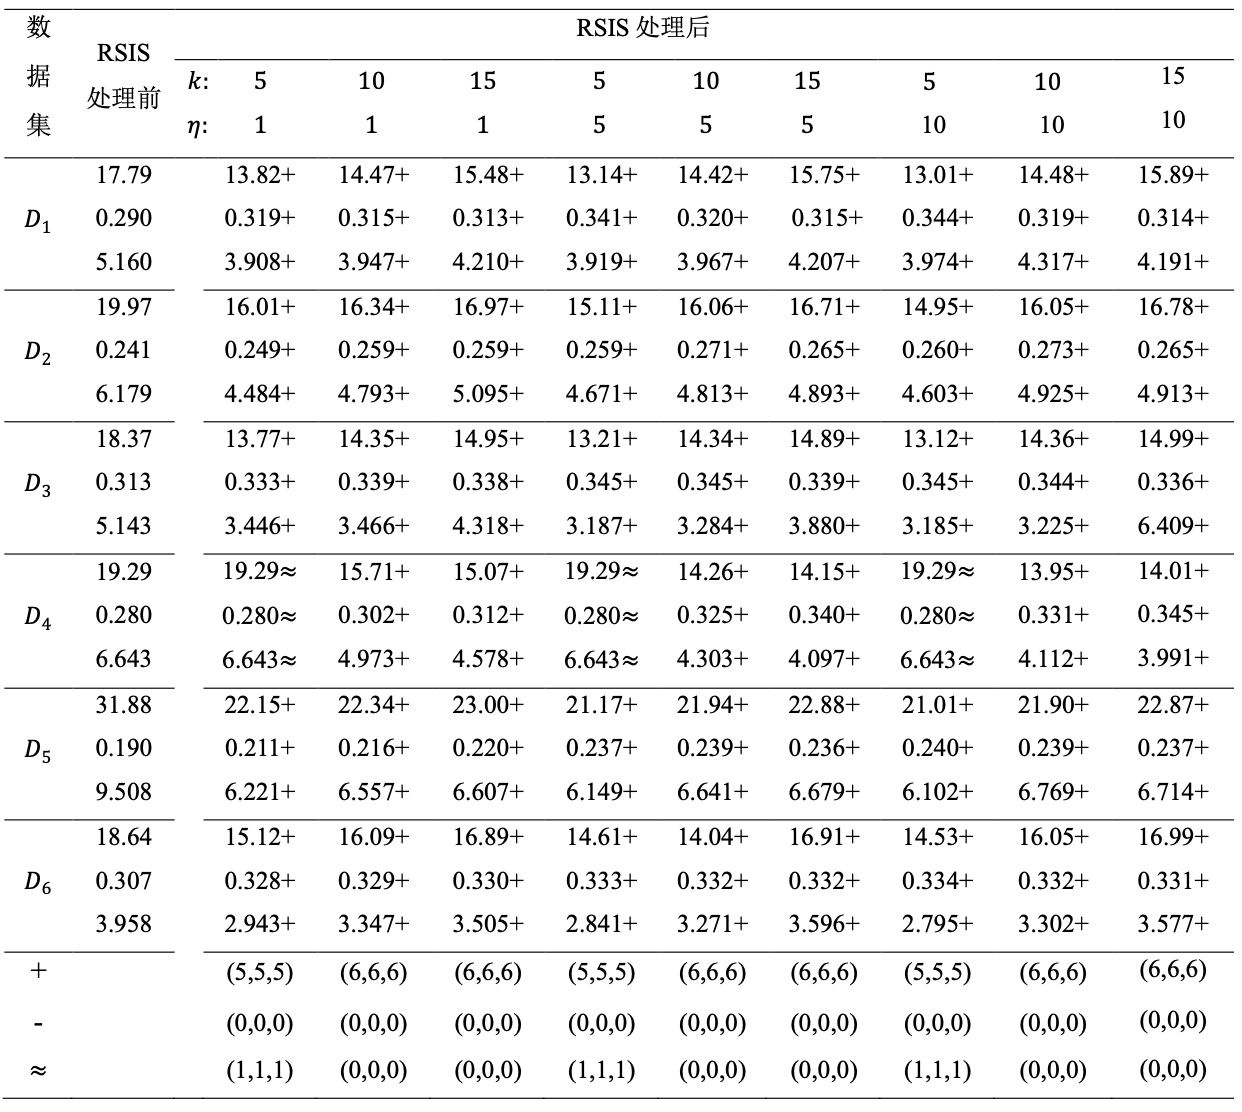
\includegraphics[width=1.0\textwidth]{figs/tab3.png}
    \label{tab3}
\end{figure}

根据实验结果可知,大多数情况下原始数据集经过RSIS方法处理后各项指标均得到了显著优化,并为存在显著恶化的情况。注意到数据集$D_4$,当超参数$k=5$,$\eta=1,5,10$时,各项指标未发生显著改变,这主要是因为随着特征维数的增加,大多数簇的样本在特征空间中变得过于稀疏。在KNN优化阶段,所有样本被合并到一个簇中,跳过了RSIS的后续处理阶段,因此并未合成新的样本。然而,随着超参数$k$的值增加,这一问题得到解决。
\\\hspace*{2em}相较于$\eta$,超参数$k$对于优化结果具有更强的敏感性,这一点会在后续的实验中得到验证。在超参数$k$的取值合适的情况下,随着$\eta$的增加,会进一步提升各项指标的优化效果。
\\\hspace*{2em}实验结果依旧显示,即使对于大方差噪音占比较高的情况下(见数据集$D_5$),RSIS依旧表现出良好的优化效果,这说明该方法是具有鲁棒性的。除此之外,即使面对样本量较少的数据集($D_6$)以及具有厚尾特征分布数据集($D_4$),RSIS方法也可以显著优化这些数据集。


\subsection{超参数分析}
为了更全面分析不同超参数下RSIS对原始数据集的优化效果,本文计算了优化前的指标与经过RSIS方法优化后的指标差值,这样可以更加直观分析其在不同的超参数组合下的优化效果,见图\ref{fig5}。
\begin{figure}[htbp]
    \centering
    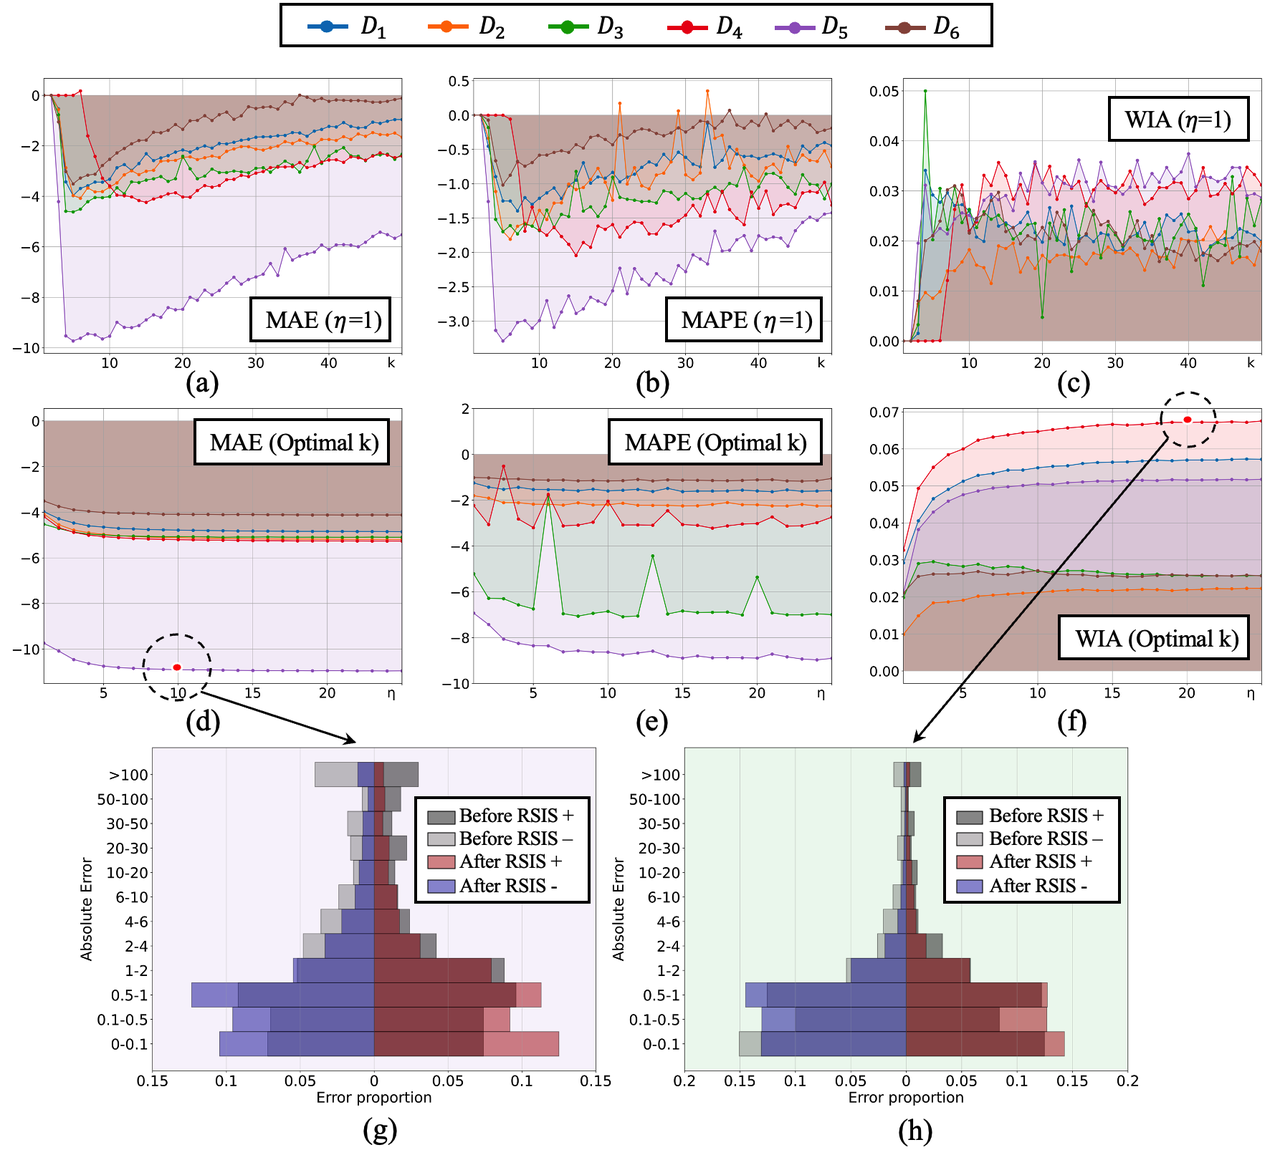
\includegraphics[width=1.0\textwidth]{figs/fig5.png}
    \caption{不同超参数下RSIS方法优化效果}
    \label{fig5}
\end{figure}
\\\hspace*{2em}图\ref{fig5}中,图(a),(b)和(c)为在超参数$\eta=1$,不同超参数$k$下三个指标的优化效果;图(d),(e)以及(f)为$k$取MAE指标最优情况下,不同超参数$\eta$下RSIS方法的优化效果;图(g)以及(h)为不同大小误差在RSIS优化前后占总样本的比例。
\\\hspace*{2em}相比MAE以及WIA,MAPE具有更大的波动性,这主要是因为RSIS合成了更多真实值接近0的样本,而MAPE指标对于真实值接近0的样本异常敏感,这在数据集$D_3$中表现更加明显。
\\\hspace*{2em}在不同的超参数$k$下,RSIS方法对于MAE以及MAPE的优化效果呈现U形,WIA会快速趋向于一个稳定的范围小幅度。
\\\hspace*{2em}相比于超参数$k$,超参数$\eta$对于优化效果的影响更加稳定。在大多数情况下,随着超参数$\eta$的增加,各项指标的优化效果会得到进一步提升。
\\\hspace*{2em}通过图(g)以及图(h)可以看出,经过RSIS方法优化后,噪音较大的样本占比明显下降,噪音较小的样本占比提升。

\section{实例分析}
\subsection{数据集介绍}
本文使用四个实例数据集去检验RSIS方法对于预测模型的优化表现\cite{ref83,ref84,ref85,ref86},具体如下:
\\\hspace*{2em}"Bike Sharing Demand"数据集是专为预测城市自行车共享系统中的租赁需求而设计的,其数据源自华盛顿特区的Capital Bikeshare程序,覆盖了2011年至2012年期间的细致使用记录。这个数据集详细记录了每小时的租赁活动,同时附有天气情况、日期和时间等相关信息。具体而言,数据集涵盖了季节变化(春、夏、秋、冬)、是否为假期、是否为工作日、以及四种不同的天气情况,从晴朗到大雨或雪。此外,每个时间点的温度、湿度、风速等气象信息也被包括在内,旨在帮助参赛者通过这些信息预测每小时的自行车租赁数量。
\\\hspace*{2em}"Air Quality"数据集集中于环境监测,提供了详尽的空气质量指标记录,旨在评估和预测各地的空气质量状况。该数据集包含从多个监测站收集的空气污染物浓度数据,如二氧化氮($\text{NO}_2$)、颗粒物(PM10和PM2.5)、一氧化碳(CO)、臭氧($\text{O}_3$)等,这些数据通常以小时或日为单位记录。除了污染物浓度,数据集还包括温度、湿度、气压等气象条件信息。
\\\hspace*{2em}"Facebook Metrics"数据集关联于2014年某知名化妆品品牌Facebook页面发布的帖子。该数据集包含Moro等人(2016年)发布帖子前已知的7个特征和用于评估帖子影响的12个特征,以及提供了每个帖子获得用户点赞的数量。
\\\hspace*{2em}"Forest Fires"数据集是由葡萄牙的Montesinho自然公园内的森林火灾记录构成的,这个数据集广泛用于研究和分析森林火灾的发生情况与多种可能的影响因素之间的关系。该数据集包含了从1998年到2003年间,关于森林火灾的517条记录,涵盖了如气象条件(包括温度、湿度、风速和降雨量等)以及空间数据(如火灾发生的月份和星期、火灾发生的坐标位置等)。这些特征被用来预测特定条件下森林火灾的燃烧面积,是研究森林火灾行为、评估火灾风险以及制定预防措施的重要资源。通过分析这个数据集,研究人员可以构建和测试模型,以预测和理解在特定气候和地理条件下森林火灾的行为,从而有助于森林管理和火灾预防工作。
\subsection{优化效果分析}
对每个数据集,随机选择不同数量规模的样本,划分为训练集与测试集。本文对训练集数据使用RSIS方法处理,随后训练模型,并在测试集上检验模型的预测效果。对于每一组实验依旧重复25次,并取平均值作为实验结果。之后进行威尔科森符号秩检验,以检验RSIS方法是否对模型的预测性能具有优化效果。选取的机器学习模型包括:K最近邻(KNN),多层感知机(MLP),梯度提升决策树(GBDT)以及支持向量回归机(SVR)。对于需要超参数调优的模型如GBDT、KNN,多次选择不同的超参数并取最好的实验结果,SVR的核函数选择径向基函数(RBF)。此外,本文剔除了无法直接使用的数据特征,如Bike Sharing Demand数据集中的“Datetime” ,Forest Fires数据集中的“Month”等。
\\\hspace*{2em}本文选用MAE以及MAPE两个指标度量RSIS方法对于预测模型泛化能力的优化效果,原始训练集使用RSIS优化前后各个模型的预测表现如表4.4所示,其中括号内的的数据为MAPE指标的实验计算结果。
\\
\begin{figure}[htbp]
    \centering
    \caption*{表4.4\;实例数据预测模型优化效果}
    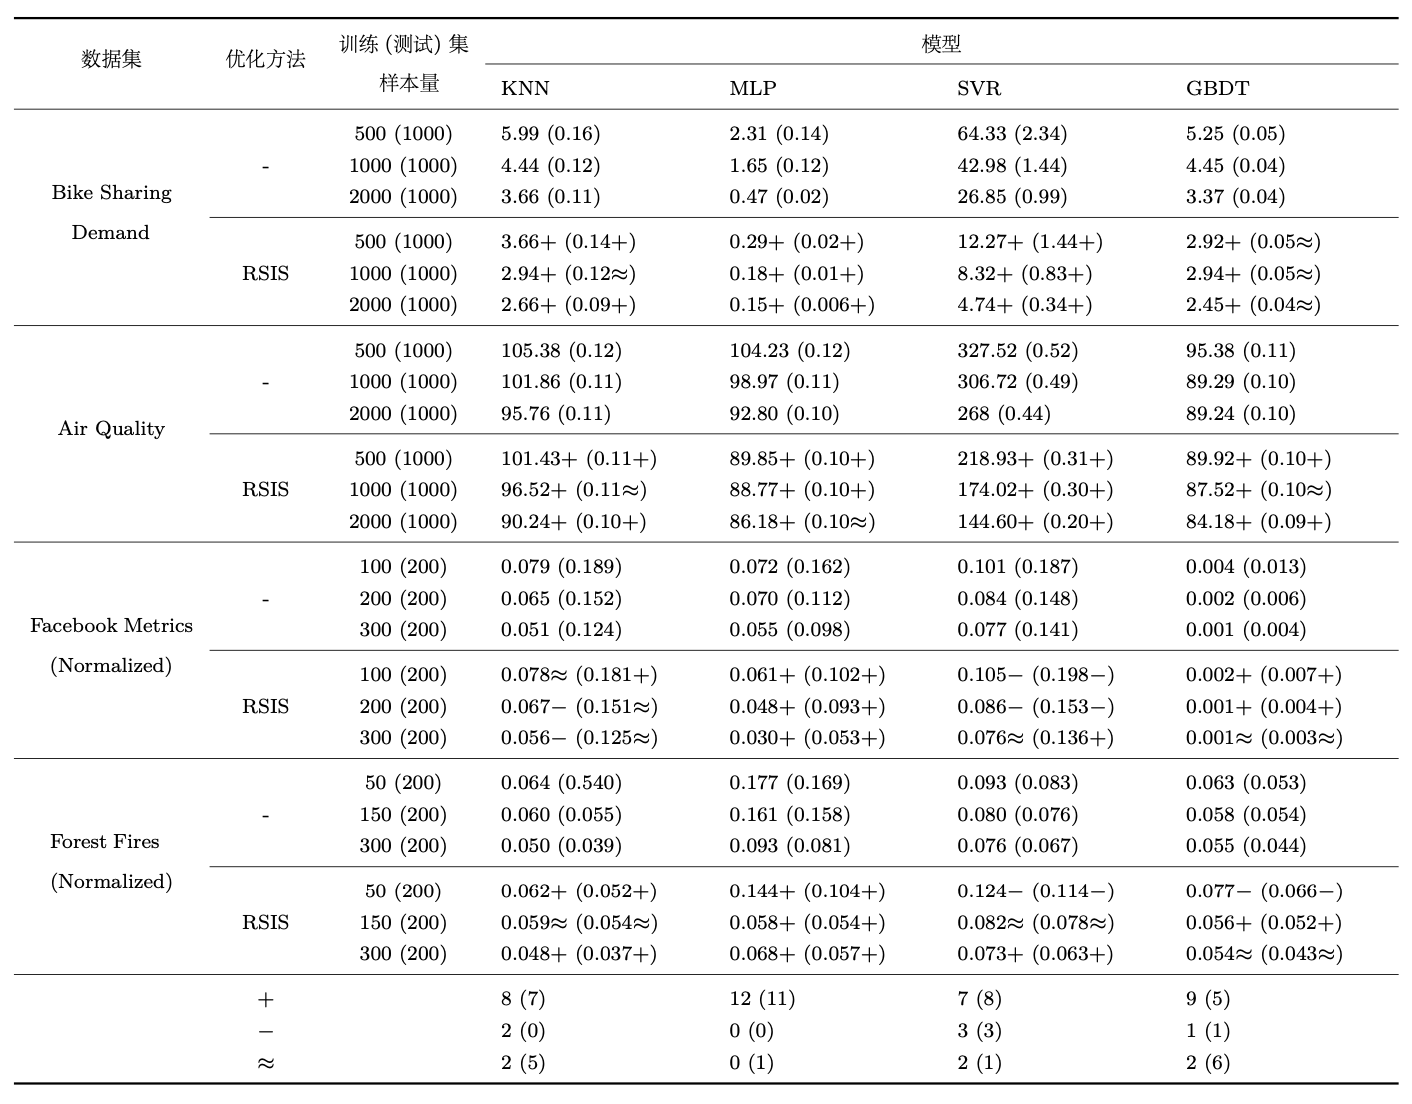
\includegraphics[width=1.0\textwidth]{figs/tab4.png}
    \label{tab4}
\end{figure}
\newpage
通过表4.4可知:
\\\hspace*{2em}1.大多数情况下RSIS方法都显著提升了模型的预测效果,对于所有的模型RSIS都表现出了良好的适应能力;
\\\hspace*{2em}2.即使针对小样本数据集以及标准化处理后的数据集,如"Facebook Metrics",RSIS依旧可以显著提升模型的预测能力;
\\\hspace*{2em}3.该部分实验并未删除掉非连续型变量的特征,这一点违背了RSIS方法变量连续的假设,并且针对样本量较少的情况,很难满足RSIS方法线性拟合函数误差趋向于0的假设。由此可见,即使违背了RSIS方法的假设,RSIS方法依旧可以对模型的预测效果显著优化,这也从另一方面体现了该方法的鲁棒性。

\begin{figure}[htbp]
    \centering
    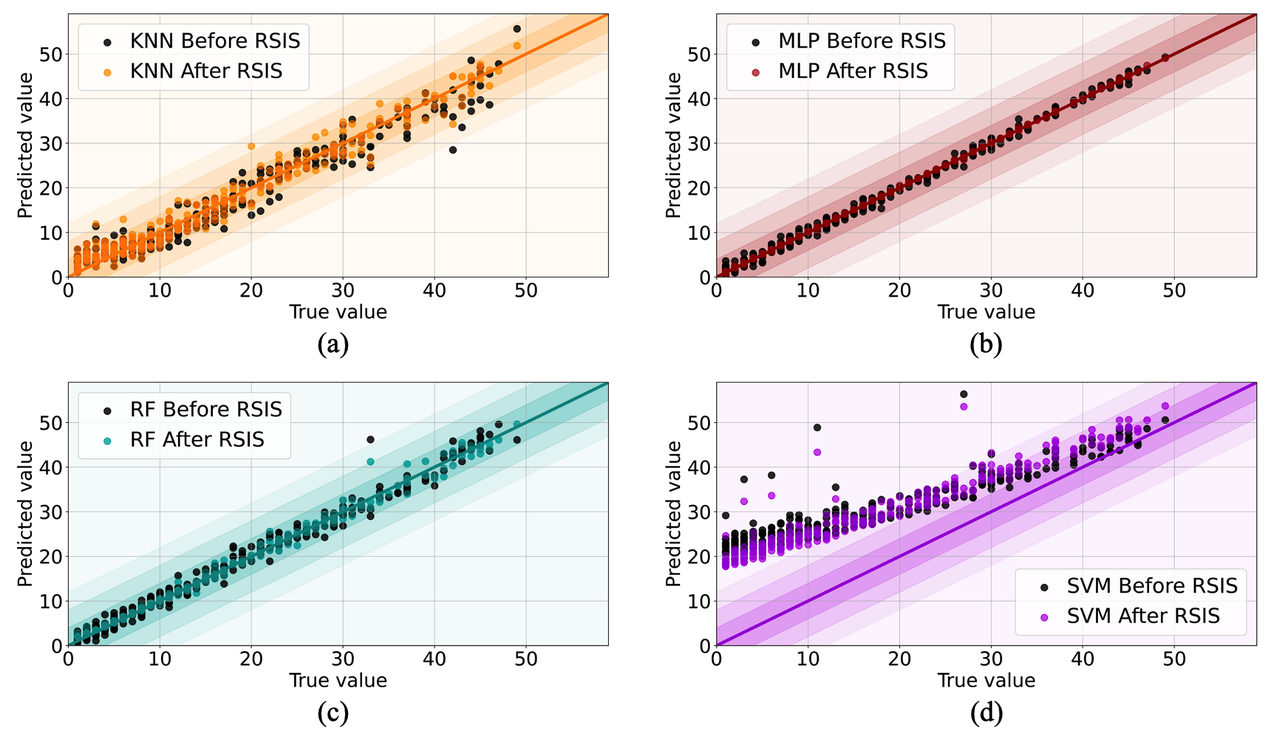
\includegraphics[width=1.0\textwidth]{figs/fig6.png}
    \caption{Bike Sharing Demand测试集上预测效果部分对比}
    \label{fig6}
\end{figure}
图\ref{fig6}展示了"Bike Sharing Demand"测试集部分样本在RSIS优化前后模型的预测值相比于真实值的差异性。可以直观的看出,经过RSIS方法优化后,模型的预测效果更加接近真实水平。

\chapter{结合卷积神经网络的进一步研究}

卷积神经网络自从在图像处理和计算机视觉领域取得突破性进展以来,已成为深度学习和人工智能研究的核心。CNN的概念最早可以追溯到20世纪60年代,但直到1980年代,由于Yann LeCun等人成功应用了卷积神经网络来识别手写数字,这标志着CNN在实际应用中的首次成功,这一方法才开始被广泛认可。自从2012年AlexNet在ImageNet挑战中大放异彩以来,CNN已经成为了计算机视觉任务中的主流方法,包括图像分类、物体检测、语义分割等。此外,CNN的应用范围已经扩展到许多其他领域,如自然语言处理(NLP)、语音识别、医学图像分析等。例如,在NLP中,CNN被用于句子分类、情感分析等任务;在医学图像分析中,CNN帮助诊断疾病、辅助手术规划。CNN商业应用中发挥着越来越重要的作用,从改进搜索引擎的图像搜索功能到支持自动驾驶汽车的视觉系统,再到提高社交媒体平台上的内容可访问性。CNN的发展标志着深度学习领域的巨大潜力,并继续推动着人工智能技术的前进。
\\\hspace*{2em}RSIS方法针对向量数据进行数据合成,但是无法直接用于图像数据,因此RSIS方法存在一定的局限性。CNN作为优秀的特征提取模型,本文将RSIS方法与传统的深度学习CNN框架相结合,提出了一种创新的CNN框架,旨在增强图像数据的特征表示和模型泛化能力。该框架首先利用CNN的卷积和池化层对输入图像进行特征提取,然后通过全局池化层将这些特征转换为一维向量表示。在此基础上,应用RSIS方法来生成新的向量表示,见图\ref{fig10}。
\\
\begin{figure}[htbp]
    \centering
    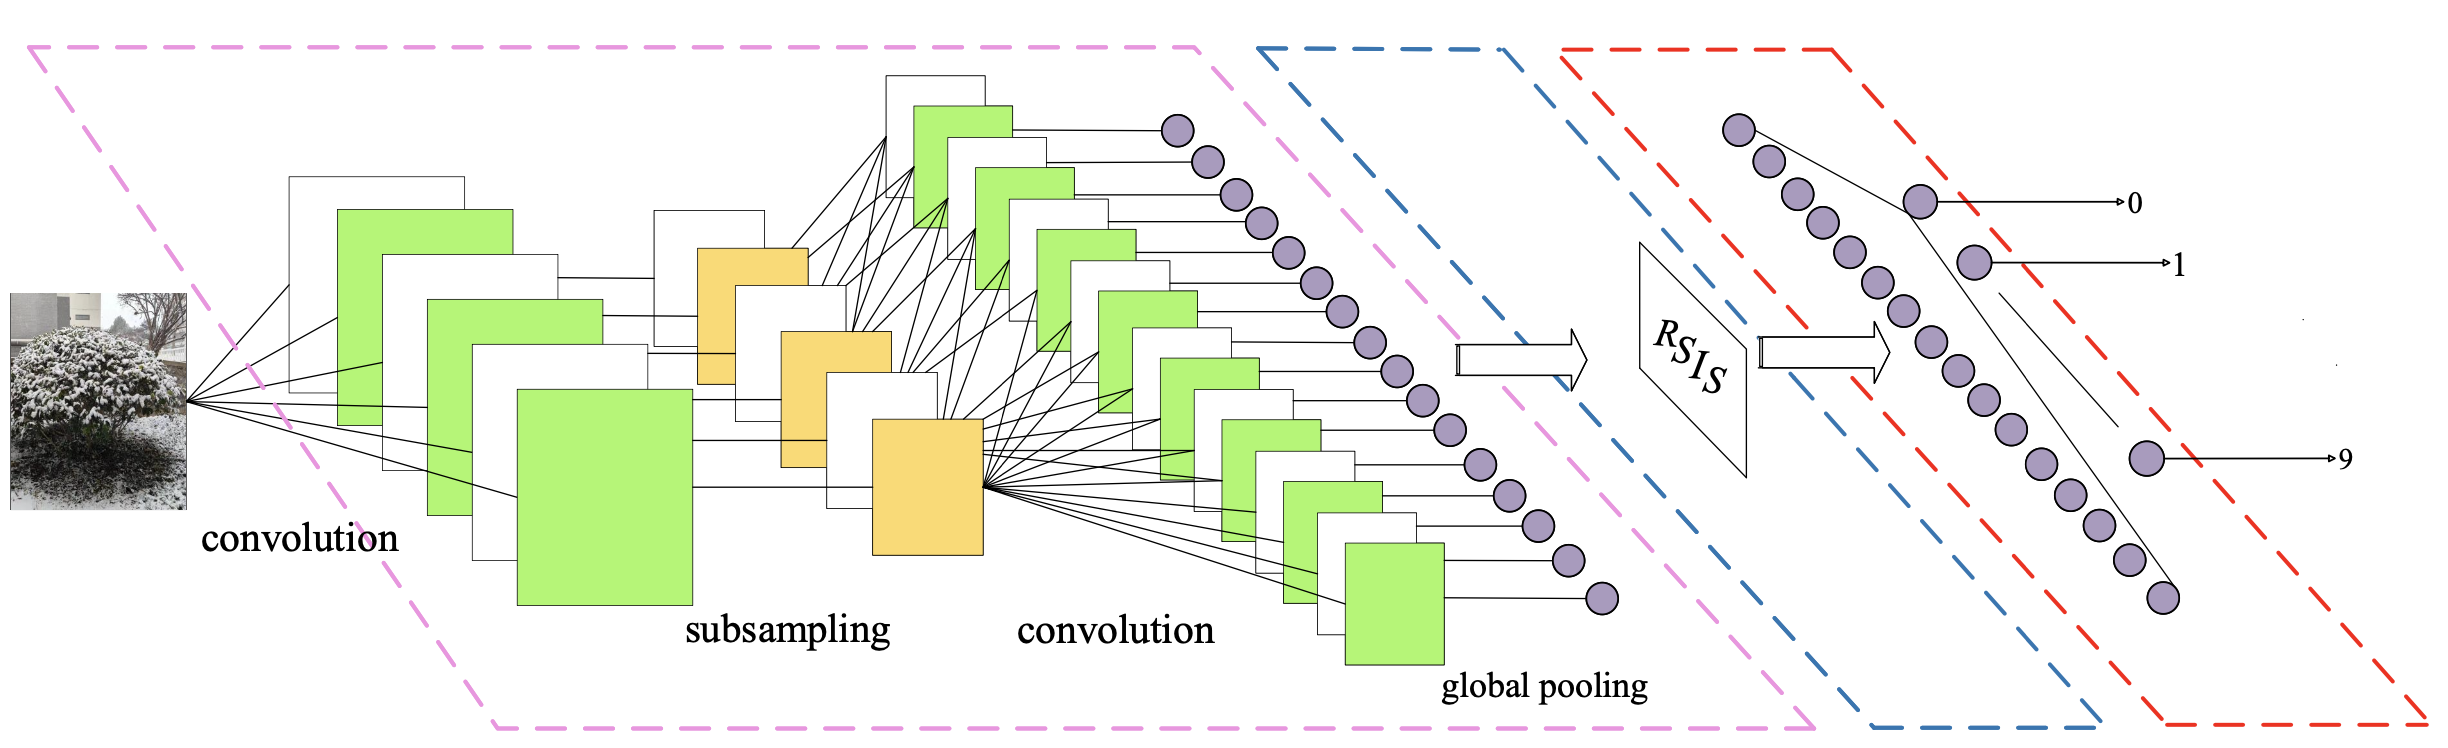
\includegraphics[width=1.0\textwidth]{figs/fig10.png}
    \caption{RSIS方法与CNN框架结合图}
    \label{fig10}
\end{figure}

\newpage
\section{方法概述}
给定一个RGB图像数据集$D=\{\boldsymbol{I}_i,L_i \}_{i=1}^n$,其中,$L_i$是反映了图像类别的独热编码向量。定义CNN的特征提取函数$f:\mathbb{R}^{H\times W\times C}\rightarrow \mathbb{R}^d$,其中$H\times W\times C$分别表示图像的高、宽以及通道数量。
通过CNN的特征提取处理,一个图像数据$\boldsymbol{I}_i$可以转化为一个特征向量,即$\boldsymbol{v}_i=f(\boldsymbol{I}_i)$。对数据集$\{\boldsymbol{v}_i,L_i \}_{i=1}^n$使用RSIS方法处理得到$\{\boldsymbol{v}_i,L_i\}_{i=1}^{n^\prime}$,其中$n^\prime$表示通过RSIS合成新的样本后添加至原始数据集的样本量。
最后将所有样本放入全连接网络中进行迭代训练。但与传统的训练方法不同,本文提出了针对该框架的两阶段模型训练方法,见图\ref{fig7}。
\\\hspace*{2em}在第一阶段中,与传统的训练方式一样,依旧将图像进行数据增强处理,随后放入模型中进行前向传播计算损失函数。最后对损失函数求梯度进行反向传播操作,更新模型参数,直至模型收敛为止。
\\

\begin{figure}[htbp]
    \centering
    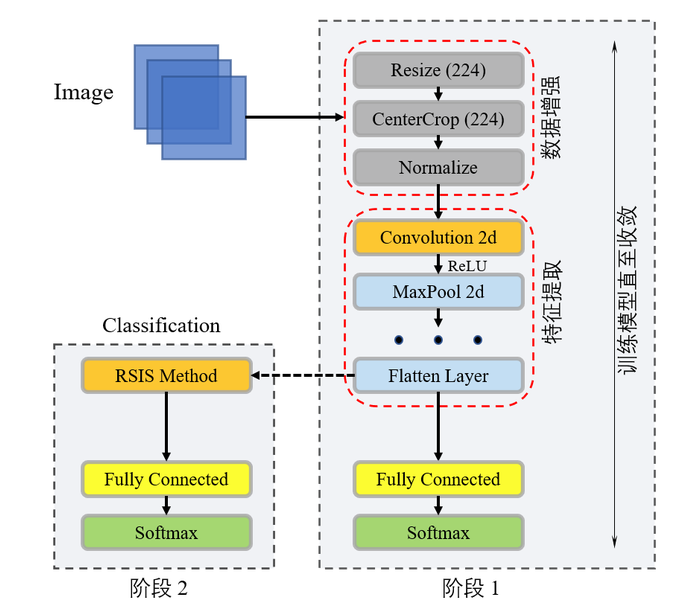
\includegraphics[width=1.0\textwidth]{figs/fig7.png}
    \caption{结合CNN框架的训练流程}
    \label{fig7}
\end{figure}


\newpage
在第二阶段中,将原始图像放入第一阶段训练好的特征提取器中得到每个图像的特征向量数据集,对特征向量数据集使用RSIS方法合成新的数据,并将新的数据再次放入全连接层中对其进行训练直到收敛。需要注意的是,这一阶段仅仅只针对全连接层的参数进行更新,特征提取层并不参与训练过程。

\section{数据集及模型网络介绍}


本文选择了四个图像数据集进行研究,包括:MNIST \cite{ref87}, FashionMNIST \cite{ref88}, CIFAR-10 \cite{ref89}以及SVHN \cite{ref90}:
\\\hspace*{2em}MNIST:手写数字数据集,包含60,000个训练样本和10,000个测试样本,图像为28x28的灰度图。
\\\hspace*{2em}FashionMNIST:服装图像数据集,结构与MNIST相同,旨在替代传统的手写数字识别任务。
\\\hspace*{2em}CIFAR-10:含有10个类别的小图像数据集,每个类别有6,000个图像,总共有50,000个训练图像和10,000个测试图像,图像尺寸为32x32彩色图。
\\\hspace*{2em}SVHN:街景房屋数字数据集,包含超过600,000个数字图像,用于数字识别任务。
\\\hspace*{2em}CNN模型选择:ResNet50, VGG16, DenseNet121, 以及 {MobileNetv2}, 所有模型均使用了预训练权重:
\\\hspace*{2em}ResNet50是残差网络(ResNet)系列中的一个变种,具有50层深的架构。它通过引入“残差块”来解决深层网络训练中的梯度消失问题,允许网络学习恒等映射,从而使得更深层次的网络训练成为可能。其准确率高,深度较大,参数数量较多,适用于复杂的图像识别任务。
\\\hspace*{2em}VGG16是视觉几何组(Visual Geometry Group)开发的卷积神经网络模型之一,特点是其均匀的架构,包含16层网络,主要由卷积层和全连接层构成。结构简单,层数较深,参数量大,计算成本较高,但模型解释性好,适用于图像识别和图像分类任务。
\\\hspace*{2em}DenseNet121是密集连接网络(DenseNet)系列中的典型代表网络,具有121层。它的特点是每一层都与前面的所有层相连接,极大地提高了网络的参数效率。其参数效率高,具有很强的特征提取能力,通过特征重用减少了模型的复杂度和计算量。
\\\hspace*{2em}MobileNetv2是专为移动和嵌入式视觉应用设计的轻量级深度学习模型。它引入了倒置残差结构,其中包括线性瓶颈层,以改进模型效率。其模型小巧,计算效率高,非常适合在计算资源有限的设备上运行,如智能手机和其他移动设备。


\section{针对CNN模型预测的优化效果分析}

对于每个数据集,分别随机选取了200以及1000个图像样本作为训练集以及测试集,在第二个阶段中,选择将训练集数据通过RSIS方法合成新的样本扩充至500,1000以及3000以探究不同的扩充规模下RSIS方法对于预测效果的优化提升。
每次实验依旧进行25次并取均值作为实验结果,同样对结果进行符号秩检验。将RSIS优化前后的错误率的差值作为度量指标以检验RSIS的优化效果,见公式\eqref{equ19}以及\eqref{equ20}。

\begin{equation}\label{equ19}
    E=\dfrac{1}{n}\sum\limits_{i=1}^n{I}(\hat{L}_i\neq L_i),
\end{equation}

\begin{equation}\label{equ20}
    E_{\text{var}}=E_{\text{stage1}}-E_{\text{stage2}},
\end{equation}
其中,$E_{\text{stage1}}$表示第一阶段结束时模型的预测错误率,$E_{\text{stage2}}$表示第二阶段后预测错误率。
\\\hspace*{2em}通过表5.1可以看出,RSIS在大多数情况下多CNN模型的预测效果都进行了显著的优化。
整体而言,RSIS方法依旧可以很好适配这些模型,对于ResNet50的优化效果提升最显著。并且优化幅度随着RSIS优化后的样本量增加而提升,这一点在MNIST以及FashionMNIST数据集表现更加明显。即使对于轻量型的网络,如MobileNetv2,RSIS也存在显著的优化效果。

\begin{figure}[htbp]
    \centering
    \label{tab5}
    \caption*{表5.1 RSISCNN网络预测优化效果}
    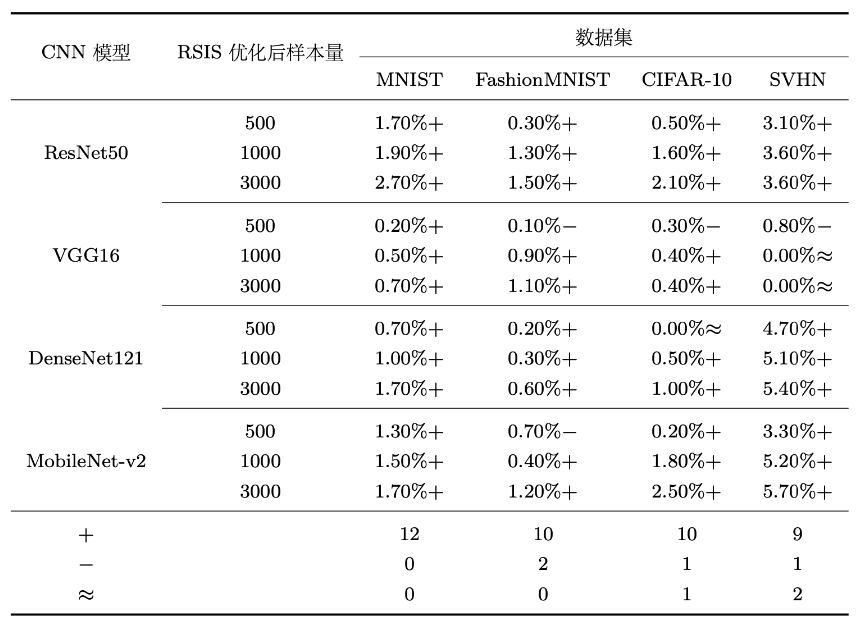
\includegraphics[width=0.9\textwidth]{figs/tab5.png}
\end{figure}

\newpage
本文选择MNIST数据集,探究不同模型随着迭代的进行$E_{\text{stage2}}$指标在测试集上的变化,如图\ref{fig8}所示,
红色虚线表示第二阶段模型训练的起始点。可以明显看出,经过RSIS优化后,不同模型在不同的优化合成的样本量下,测试集上的$E_{\text{stage2}}$均有所下降。

\begin{figure}[htbp]
    \centering
    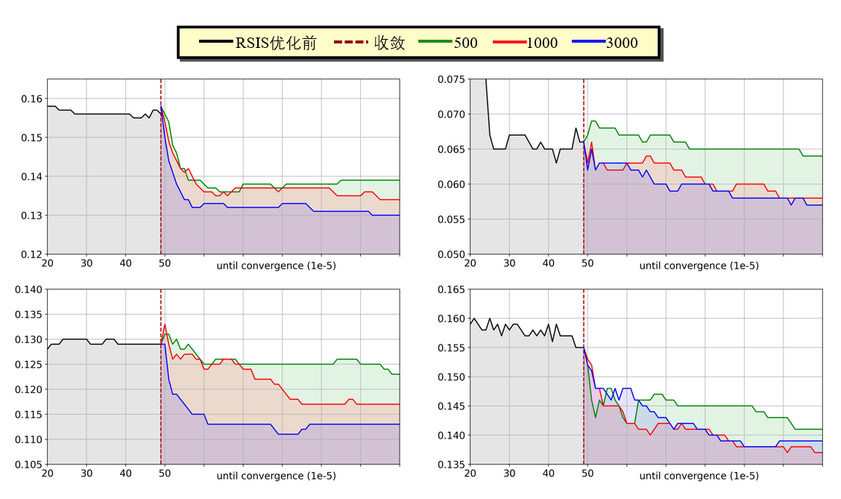
\includegraphics[width=1.0\textwidth]{figs/fig8.png}
    \caption{随着迭代进行$E_{\text{stage2}}$在测试集上变化}
    \label{fig8}
\end{figure}

\begin{figure}[htbp]
    \centering
    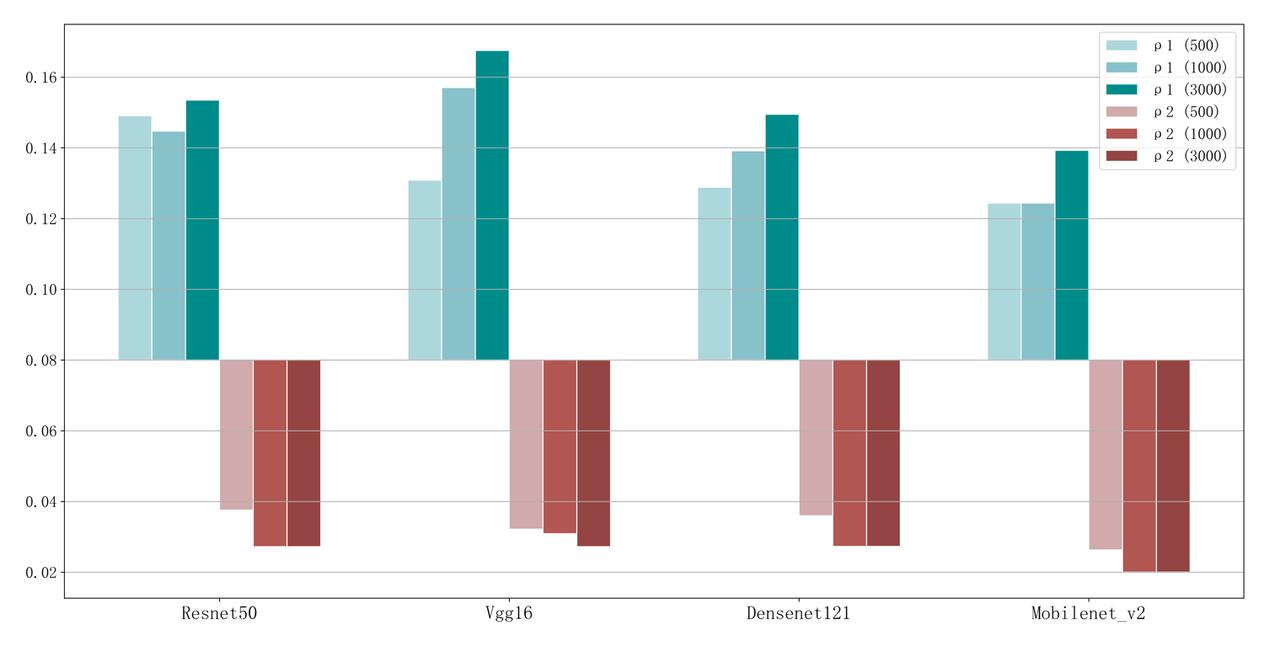
\includegraphics[width=1.0\textwidth]{figs/fig9.png}
    \caption{RSIS优化前后$\rho_1$,$\rho_2$指标对比}
    \label{fig9}
\end{figure}

图\ref{fig9}展示了FashionMNIST数据集在RSIS优化前后指标$\rho_1$(误分类改进比)以及指标$\rho_2$(负转化率)的对比表现:

\begin{equation}\label{equ21}
    \rho_1=\dfrac{\text{num}(C_{\text{stage2}}\cap  M_{\text{stage1}})}{\text{num}(M_{\text{stage1}})},
\end{equation}

\begin{equation}\label{equ22}
    \rho_2=\dfrac{\text{num}(M_{\text{stage2}}\cap C_{\text{stage1}})}{\text{num}(C_{\text{stage1}})},
\end{equation}

其中,$M_{\text{stage1}}$以及$M_{\text{stage2}}$分别为在RSIS优化前后测试集上错误分类的图像集合,$C_{\text{stage1}}$以及$C_{\text{stage2}}$为RSIS优化前后测试集上正确分类的图像集合。
简单来说,$\rho_1$反映了经过RSIS优化后,原本被误分类的样本中有多少比例被纠正;而$\rho_2$表示了经过优化后,原本正确分类的样本中有多少变成了误分类。在优化方法性能评估中,$\rho_1$较高意味着模型在识别之前误分类的样本方面有显著提升,而$\rho_2$较低则表明模型稳定性较好,优化过程中没有引入过多新的误分类。
\\\hspace*{2em}在大多数情况下,随着训练集中合成样本数量的增加,$\rho_1$往往呈上升趋势,这一趋势在VGG16和DenseNet121中尤为明显;相反,$\rho_2$通常随着训练集的扩大而减小,这一现象在VGG16中特别显著。

\chapter{总结与展望}
本文提出了一种创新的对于含噪数据集优化的数据合成方法,基于特征子空间插值的思想,命名为RSIS方法。该方法可以在保证不损害样本原始信息的前提下,合成大量具有较小误差的样本,从而提升机器学习模型的泛化能力。本文对RSIS方法进行了全面的模拟研究,通过生成含有复杂且未知噪音的数据集,实验结果表明了RSIS方法对于含噪数据集具有显著的优化效果。在实例数据中,将经过RSIS优化后的样本用于机器学习实际的预测场景中,实验结果表明该方法可以显著提升模型的泛化能力。并且本文还将RSIS方法应用到计算机视觉领域进行拓展研究,创新地RSIS方法与卷积神经网络相结合,该部分的实验同样表明RSIS方法依旧可以显著提升模型在图像分类任务的预测效果。
\\\hspace*{2em}然而,该方法也存在一定不足。首先,通过这种子空间插值的数据合成方式会破坏原始样本的分布信息,从理论上讲,若超参数$\eta$取无穷大,则样本的特征会呈现均匀分布;其次,该方法对于超参数$k$较为敏感,参数寻优的过程并没有严谨,且可以自适应寻优的方法;最后,RSIS方法有严格的前提假设,尽管本文在实验中验证了违背该方法假设情况下的鲁棒性,但是并不能保证RSIS方法在许多实际任务场景中可以完全适用。
\\\hspace*{2em}在未来的研究中,一方面,RSIS方法的自适应超参数优化是值得进一步研究的方向,这可以节省大量的调参工作使得该方法更加便捷高效;除此之外,也可以将RSIS方法的思想用于全局优化算法的研究,比如遗传算法、差分进化算法等,作为一种独特的变异策略在搜索空间中合成更多的个体进行全局寻优;最后,RSIS方法受限于数据集变量属性,拓宽RSIS方法的适用性,如何将RSIS方法用于含有离散特征变量的样本进行数据合成也是未来值得探究的方向。


\begin{thebibliography}{99}
\setlength{\baselineskip}{10pt}{\setlength\arraycolsep{2pt}}
\bibitem{ref1}
杜玉坤,金骁,汪红霞. 一种基于自适应子空间线性插值的数据合成方法[C]. 国防科技大学系统工程学院. 第五届体系工程学术会议论文集——数智时代的体系工程. 2023: 16.
\bibitem{ref2}
蒋远,牟辰光,苏小红等. 噪音过滤和深度学习相结合的安全缺陷报告识别 [J]. 计算机学报, 2022, 45 (08): 1794-1813.
\bibitem{ref3}
汪红霞, 金骁, 杜玉坤, 张楠. 基于多任务深度学习的自适应软参数共享方法. 系统科学与数学, 2024, 44(2): 551-566 
\bibitem{ref4}
Karimi D, Dou H, Warfield S K, et al. Deep learning with noisy labels: Exploring techniques and remedies in medical image analysis[J]. Medical image analysis, 2020, 65: 101759.
\bibitem{ref5}
Sikder M N K, Batarseh F A. Outlier detection using AI: a survey[J]. AI Assurance, 2023: 231-291.
\bibitem{ref6}
Ullo S L, Sinha G R. Advances in smart environment monitoring systems using IoT and sensors[J]. Sensors, 2020, 20(11): 3113.
\bibitem{ref7}
Chu X, Ilyas I F, Krishnan S, et al. Data cleaning: Overview and emerging challenges[C]//Proceedings of the 2016 international conference on management of data. 2016: 2201-2206
\bibitem{ref8}
Berti-Equille L, Dasu T, Srivastava D. Discovery of complex glitch patterns: A novel approach to quantitative data cleaning[C]//2011 IEEE 27th International Conference on Data Engineering. IEEE, 2011: 733-744.
\bibitem{ref9}
Buades A, Coll B, Morel J M. Non-local means denoising[J]. Image Processing On Line, 2011, 1: 208-212.
\bibitem{ref10}
Wink A M, Roerdink J B T M. Denoising functional MR images: a comparison of wavelet denoising and Gaussian smoothing[J]. IEEE transactions on medical imaging, 2004, 23(3): 374-387.
\bibitem{ref11}
Lukasik M, Bhojanapalli S, Menon A, et al. Does label smoothing mitigate label noise?[C]//International Conference on Machine Learning. PMLR, 2020: 6448-6458.
\bibitem{ref12}
Liguori C, Paolillo A, Ruggiero A, et al. Outlier detection for the evaluation of the measurement uncertainty of environmental acoustic noise[J]. IEEE Transactions on Instrumentation and Measurement, 2015, 65(2): 234-242.
\bibitem{ref13}
Takahashi K, Ooka R, Kurosaki A. Seasonal threshold to reduce false positives for prediction-based outlier detection in building energy data[J]. Journal of Building Engineering, 2024, 84: 108539.
\bibitem{ref14}
Osborne J W. Best practices in data cleaning: A complete guide to everything you need to do before and after collecting your data[M]. Sage publications, 2012.
\bibitem{ref15}
Ma J, Zou Y, Tang X, et al. Spatial Pooling Transformer Network and Noise-Tolerant Learning for Noisy Hyperspectral Image Classification[J]. IEEE Transactions on Geoscience and Remote Sensing, 2024.
\bibitem{ref16}
Nie D, Trullo R, Lian J, et al. Medical image synthesis with deep convolutional adversarial networks[J]. IEEE Transactions on Biomedical Engineering, 2018, 65(12): 2720-2730.
\bibitem{ref17}
Goncalves A, Ray P, Soper B, et al. Generation and evaluation of synthetic patient data[J]. BMC medical research methodology, 2020, 20: 1-40.
\bibitem{ref18}
Gautschi W. Numerical analysis[M]. Springer Science \& Business Media, 2011.
\bibitem{ref19}
Lewis J P. Algorithms for solid noise synthesis[C]//Proceedings of the 16th annual conference on Computer graphics and interactive techniques. 1989: 263-270.
\bibitem{ref20}
Zhang H, Cisse M, Dauphin Y N, et al. mixup: Beyond empirical risk minimization[J]. arXiv preprint arXiv:1710.09412, 2017.
\bibitem{ref21}
Walawalkar D, Shen Z, Liu Z, et al. Attentive cutmix: An enhanced data augmentation approach for deep learning based image classification[J]. arXiv preprint arXiv:2003.13048, 2020.
\bibitem{ref22}
Robert C P, Casella G, Casella G. Monte Carlo statistical methods[M]. New York: Springer, 1999.
\bibitem{ref23}
Queipo N V, Haftka R T, Shyy W, et al. Surrogate-based analysis and optimization[J]. Progress in aerospace sciences, 2005, 41(1): 1-28.
\bibitem{ref24}
Bhosekar A, Ierapetritou M. Advances in surrogate based modeling, feasibility analysis, and optimization: A review[J]. Computers \& Chemical Engineering, 2018, 108: 250-267.
\bibitem{ref25}
Nasios N, Bors A G. Variational learning for Gaussian mixture models[J]. IEEE Transactions on Systems, Man, and Cybernetics, Part B (Cybernetics), 2006, 36(4): 849-862.
\bibitem{ref26}
Friedman N, Goldszmidt M, Lee T J. Bayesian Network Classification with Continuous Attributes: Getting the Best of Both Discretization and Parametric Fitting[C]//ICML. 1998, 98: 179-187.
\bibitem{ref27}
Arandjelovic O, Cipolla R. Incremental learning of temporally-coherent gaussian mixture models[J]. 2005.
\bibitem{ref28}
Achlioptas P, Diamanti O, Mitliagkas I, et al. Learning representations and generative models for 3d point clouds[C]//International conference on machine learning. PMLR, 2018: 40-49.
\bibitem{ref29}
Raab G M, Nowok B, Dibben C. Practical data synthesis for large samples[J]. Journal of Privacy and Confidentiality, 2016, 7(3): 67-97.
\bibitem{ref30}
Ling H, Okada K. Diffusion distance for histogram comparison[C]//2006 IEEE Computer Society Conference on Computer Vision and Pattern Recognition (CVPR'06). IEEE, 2006, 1: 246-253.
\bibitem{ref31}
Oyang Y J, Hwang S C, Ou Y Y, et al. Data classification with radial basis function networks based on a novel kernel density estimation algorithm[J]. IEEE transactions on neural networks, 2005, 16(1): 225-236.
\bibitem{ref32}
Chawla N V, Bowyer K W, Hall L O, et al. SMOTE: synthetic minority over-sampling technique[J]. Journal of artificial intelligence research, 2002, 16: 321-357.
\bibitem{ref33}
Tang Y, Zhang Y Q, Chawla N V, et al. SVMs modeling for highly imbalanced classification[J]. IEEE Transactions on Systems, Man, and Cybernetics, Part B (Cybernetics), 2008, 39(1): 281-288.
\bibitem{ref34}
Mukherjee M, Khushi M. SMOTE-ENC: A novel SMOTE-based method to generate synthetic data for nominal and continuous features[J]. Applied System Innovation, 2021, 4(1): 18.
\bibitem{ref35}
Salimans T, Goodfellow I, Zaremba W, et al. Improved techniques for training gans[J]. Advances in neural information processing systems, 2016, 29.
\bibitem{ref36}
Alqahtani H, Kavakli-Thorne M, Kumar G. Applications of generative adversarial networks (gans): An updated review[J]. Archives of Computational Methods in Engineering, 2021, 28: 525-552.
\bibitem{ref37}
Creswell A, White T, Dumoulin V, et al. Generative adversarial networks: An overview[J]. IEEE signal processing magazine, 2018, 35(1): 53-65.
\bibitem{ref38}
Bond-Taylor S, Leach A, Long Y, et al. Deep generative modelling: A comparative review of vaes, gans, normalizing flows, energy-based and autoregressive models[J]. IEEE transactions on pattern analysis and machine intelligence, 2021, 44(11): 7327-7347.
\bibitem{ref39}
Sohn K, Lee H, Yan X. Learning structured output representation using deep conditional generative models[J]. Advances in neural information processing systems, 2015, 28.
\bibitem{ref40}
Li M, Lin J, Ding Y, et al. Gan compression: Efficient architectures for interactive conditional gans[C]//Proceedings of the IEEE/CVF conference on computer vision and pattern recognition. 2020: 5284-5294.
\bibitem{ref41}
Isola P, Zhu J Y, Zhou T, et al. Image-to-image translation with conditional adversarial networks[C]//Proceedings of the IEEE conference on computer vision and pattern recognition. 2017: 1125-1134.
\bibitem{ref42}
Van Den Oord A, Kalchbrenner N, Kavukcuoglu K. Pixel recurrent neural networks[C]//International conference on machine learning. PMLR, 2016: 1747-1756.
\bibitem{ref43}
Nguyen A, Clune J, Bengio Y, et al. Plug \& play generative networks: Conditional iterative generation of images in latent space[C]//Proceedings of the IEEE conference on computer vision and pattern recognition. 2017: 4467-4477.
\bibitem{ref44}
Salimans T, Karpathy A, Chen X, et al. Pixelcnn++: Improving the pixelcnn with discretized logistic mixture likelihood and other modifications[J]. arXiv preprint arXiv:1701.05517, 2017.
\bibitem{ref45}
Elguebaly T, Bouguila N. Bayesian learning of finite generalized Gaussian mixture models on images[J]. Signal Processing, 2011, 91(4): 801-820.
\bibitem{ref46}
Roberts S J, Husmeier D, Rezek I, et al. Bayesian approaches to Gaussian mixture modeling[J]. IEEE Transactions on Pattern Analysis and Machine Intelligence, 1998, 20(11): 1133-1142.
\bibitem{ref47}
Xu H, Zha H. A dirichlet mixture model of hawkes processes for event sequence clustering[J]. Advances in neural information processing systems, 2017, 30.
\bibitem{ref48}
Bouguila N, Ziou D. A Dirichlet process mixture of generalized Dirichlet distributions for proportional data modeling[J]. IEEE Transactions on Neural Networks, 2009, 21(1): 107-122.
\bibitem{ref49}
Eddy S R. Accelerated profile HMM searches[J]. PLoS computational biology, 2011, 7(10): e1002195.
\bibitem{ref50}
Hong S, Yang D, Choi J, et al. Inferring semantic layout for hierarchical text-to-image synthesis[C]//Proceedings of the IEEE conference on computer vision and pattern recognition. 2018: 7986-7994.
\bibitem{ref51}
Jordon J, Yoon J, Van Der Schaar M. PATE-GAN: Generating synthetic data with differential privacy guarantees[C]//International conference on learning representations. 2018.
\bibitem{ref52}
Breunig M M, Kriegel H P, Ng R T, et al. LOF: identifying density-based local outliers[C]//Proceedings of the 2000 ACM SIGMOD international conference on Management of data. 2000: 93-104.
\bibitem{ref53}
Reinelt G. The traveling salesman: computational solutions for TSP applications[M]. Springer, 2003.
\bibitem{ref54}
Shi X H, Liang Y C, Lee H P, et al. Particle swarm optimization-based algorithms for TSP and generalized TSP[J]. Information processing letters, 2007, 103(5): 169-176.
\bibitem{ref55}
Jünger M, Reinelt G, Rinaldi G. The traveling salesman problem[J]. Handbooks in operations research and management science, 1995, 7: 225-330.
\bibitem{ref56}
Razali N M, Geraghty J. Genetic algorithm performance with different selection strategies in solving TSP[C]//Proceedings of the world congress on engineering. Hong Kong, China: International Association of Engineers, 2011, 2(1): 1-6.
\bibitem{ref57}
Matai R, Singh S P, Mittal M L. Traveling salesman problem: an overview of applications, formulations, and solution approaches[J]. Traveling salesman problem, theory and applications, 2010, 1(1): 1-25.
\bibitem{ref58}
Arora S. Polynomial time approximation schemes for Euclidean TSP and other geometric problems[C]//Proceedings of 37th Conference on Foundations of Computer Science. IEEE, 1996: 2-11.
\bibitem{ref59}
Birattari M, Balaprakash P, Stützle T, et al. Estimation-based local search for stochastic combinatorial optimization using delta evaluations: a case study on the probabilistic traveling salesman problem[J]. INFORMS Journal on Computing, 2008, 20(4): 644-658.
\bibitem{ref60}
Barron A R, Cohen A, Dahmen W, et al. Approximation and learning by greedy algorithms[J]. 2008.
\bibitem{ref61}
Shafique K, Shah M. A noniterative greedy algorithm for multiframe point correspondence[J]. IEEE transactions on pattern analysis and machine intelligence, 2005, 27(1): 51-65.
\bibitem{ref62}
Zhang Z, Schwartz S, Wagner L, et al. A greedy algorithm for aligning DNA sequences[J]. Journal of Computational biology, 2000, 7(1-2): 203-214.
\bibitem{ref63}
Gülcü Ş, Mahi M, Baykan Ö K, et al. A parallel cooperative hybrid method based on ant colony optimization and 3-Opt algorithm for solving traveling salesman problem[J]. Soft Computing, 2018, 22: 1669-1685.
\bibitem{ref64}
Mahi M, Baykan Ö K, Kodaz H. A new hybrid method based on particle swarm optimization, ant colony optimization and 3-opt algorithms for traveling salesman problem[J]. Applied Soft Computing, 2015, 30: 484-490.
\bibitem{ref65}
Martin O, Otto S W, Felten E W. Large-step Markov chains for the traveling salesman problem[M]. Oregon Graduate Institute of Science and Technology, Department of Computer Science and Engineering, 1991.
\bibitem{ref66}
Ho J, Lee K C, Yang M H, et al. Visual tracking using learned linear subspaces[C]//Proceedings of the 2004 IEEE Computer Society Conference on Computer Vision and Pattern Recognition, 2004. CVPR 2004. IEEE, 2004, 1: I-I.
\bibitem{ref67}
Jansson M, Wahlberg B. A linear regression approach to state-space subspace system identification[J]. Signal Processing, 1996, 52(2): 103-129.
\bibitem{ref68}
Cai D, Han J. Spectral regression for efficient regularized subspace learning[C]//2007 IEEE 11th international conference on computer vision. IEEE, 2007.
\bibitem{ref69}
Sun Q, Ge Z. A survey on deep learning for data-driven soft sensors[J]. IEEE Transactions on Industrial Informatics, 2021, 17(9): 5853-5866.
\bibitem{ref70}
Kadlec P, Grbić R, Gabrys B. Review of adaptation mechanisms for data-driven soft sensors[J]. Computers \& chemical engineering, 2011, 35(1): 1-24.
\bibitem{ref71}
Stickland A C, Murray I. Bert and pals: Projected attention layers for efficient adaptation in multi-task learning[C]//International Conference on Machine Learning. PMLR, 2019: 5986-5995.
\bibitem{ref72}
Cheng Y, Wang D, Zhou P, et al. Model compression and acceleration for deep neural networks: The principles, progress, and challenges[J]. IEEE Signal Processing Magazine, 2018, 35(1): 126-136.
\bibitem{ref73}
Wang H, Jiang Z, Zhang H, et al. An integrated MCDM approach considering demands-matching for reverse logistics[J]. Journal of cleaner production, 2019, 208: 199-210.
\bibitem{ref74}
Johnson D S, Lenstra J K, Kan A H G R. The complexity of the network design problem[J]. Networks, 1978, 8(4): 279-285.
\bibitem{ref75}
Zhou Z, Liu P, Feng J, et al. Computation resource allocation and task assignment optimization in vehicular fog computing: A contract-matching approach[J]. IEEE Transactions on Vehicular Technology, 2019, 68(4): 3113-3125.
\bibitem{ref76}
Avis D. A survey of heuristics for the weighted matching problem[J]. Networks, 1983, 13(4): 475-493.
\bibitem{ref77}
Neely M. Stochastic network optimization with application to communication and queueing systems[M]. Springer Nature, 2022.
\bibitem{ref78}
Advani M S, Saxe A M, Sompolinsky H. High-dimensional dynamics of generalization error in neural networks[J]. Neural Networks, 2020, 132: 428-446.
\bibitem{ref79}
Krishnan D, Fergus R. Fast image deconvolution using hyper-Laplacian priors[J]. Advances in neural information processing systems, 2009, 22.
\bibitem{ref80}
Duan R, Pettie S. Linear-time approximation for maximum weight matching[J]. Journal of the ACM (JACM), 2014, 61(1): 1-23.
\bibitem{ref81}
Guo Y, Wang W, Wang X. A robust linear regression feature selection method for data sets with unknown noise[J]. IEEE Transactions on Knowledge and Data Engineering, 2021, 35(1): 31-44.
\bibitem{ref82}
Wu G, Mallipeddi R, Suganthan P N, et al. Differential evolution with multi-population based ensemble of mutation strategies[J]. Information Sciences, 2016, 329: 329-345.
\bibitem{ref83}
Will Cukierski. (2014). Bike Sharing Demand. Kaggle. https://kaggle.com/competitions/bike-sharing-demand.
\bibitem{ref84}
Vito,Saverio. (2016). Air Quality. UCI Machine Learning Repository. https://doi.org/10.24432/C59K5F.
\bibitem{ref85}
Moro,Srgio, Rita,Paulo, and Vala,Bernardo. (2016). Facebook Metrics. UCI Machine Learning Repository. https://doi.org/10.24432/C5QK55.
\bibitem{ref86}
Cortez,Paulo and Morais,Anbal. (2008). Forest Fires. UCI Machine Learning Repository. https://doi.org/10.24432/C5D88D. 
\bibitem{ref87}
LeCun Y, Bottou L, Bengio Y, et al. Gradient-based learning applied to document recognition[J]. Proceedings of the IEEE, 1998, 86(11): 2278-2324.
\bibitem{ref88}
Xiao H, Rasul K, Vollgraf R. Fashion-mnist: a novel image dataset for benchmarking machine learning algorithms[J]. arXiv preprint arXiv:1708.07747, 2017.
\bibitem{ref89}
Krizhevsky A, Hinton G. Learning multiple layers of features from tiny images[J]. 2009.
\bibitem{ref90}
Netzer Y, Wang T, Coates A, et al. Reading digits in natural images with unsupervised feature learning[C]//NIPS workshop on deep learning and unsupervised feature learning. 2011, 2011(5): 7.

\end{thebibliography}

\begin{ResearchAchievements}

\noindent
Liang J, Du Y, Xu Y, et al. Using Adaptive Chaotic Grey Wolf Optimization for the daily streamflow prediction[J]. Expert Systems with Applications, 2024, 237: 121113.\\ 
\\
Du Y, Cai Y, Jin X, et al. ASIDS: A Robust Data Synthesis Method for Generating Optimal Synthetic Samples[J]. Mathematics, 2023, 11(18): 3891.\\ 
\\
Du Y, Jin X, Wang H, et al. An Adaptive Multipath Linear Interpolation Method for Sample Optimization[J]. Mathematics, 2023, 11(3): 768.\\ 
\\
汪红霞, 金骁, 杜玉坤, 张楠. 基于多任务深度学习的自适应软参数共享方法. 系统科学与数学, 2024, 44(2): 551-566\\ 
\\
杜玉坤,金骁,汪红霞. 一种基于自适应子空间线性插值的数据合成方法[C]. 国防科技大学系统工程学院. 第五届体系工程学术会议论文集——数智时代的体系工程. 2023: 16.

\end{ResearchAchievements}

\begin{ThanksPage}
感谢我的硕士指导老师苍玉权、陆敏教授对我的帮助(希望毕业了以后还能多跟陆老师喝酒!);感谢汪院长对我论文的指导;感谢辅导员侯婷婷老师对我生活上遇到一些麻烦的帮助(顺便对她每天焦头烂额的忙碌表示同情);感谢和我一起撰写论文的同学蔡奕涛、金骁(按照姓氏拼音排名,不分先后);感谢褚明阳无偿资助我的咖啡和酒(其实是玩游戏输了的请客,又菜又爱玩)。哦对了,小褚马上结婚了,顺祝他幸福。
\\\hspace*{2em}最后,感谢我的父母对我各方面的支持,使我可以更加坚定学术的道路,继续读博。
\\\hspace*{2em}文末置笔,倚梦随风,酌敬南审青葱之岁月。
\end{ThanksPage}
\end{document}